\documentclass[11pt,a4paper,oneside]{report}             % Single-side
%\documentclass[11pt,a4paper,twoside,openright]{report}  % Duplex

%\PassOptionsToPackage{chapternumber=Huordinal}{magyar.ldf}
\usepackage{t1enc}
\usepackage[latin2]{inputenc}
\usepackage{amsmath}
\usepackage{amssymb}
\usepackage{algorithm}
\usepackage[noend]{algpseudocode}
\usepackage{enumerate}
\usepackage[thmmarks]{ntheorem}
\usepackage{graphics}
\usepackage{epsfig}
\usepackage{listings}
\usepackage{color}
%\usepackage{fancyhdr}
\usepackage{lastpage}
\usepackage{anysize}
\usepackage[magyar]{babel}
\usepackage{sectsty}
\usepackage{setspace}  % Ettol a tablazatok, abrak, labjegyzetek maradnak 1-es sorkozzel!
\usepackage[hang]{caption}
\usepackage{hyperref}

%--------------------------------------------------------------------------------------
% Main variables
%--------------------------------------------------------------------------------------
\newcommand{\vikszerzo}{Gurz� Lajos}
\newcommand{\vikkonzulens}{dr.~Umenhoffer Tam�s}
\newcommand{\vikcim}{�ltal�nos c�l�, komponens alap� j�t�kmotor fejleszt�se}
\newcommand{\viktanszek}{Ir�ny�t�stechnika �s Informatika Tansz�k}
\newcommand{\vikdoktipus}{Diplomaterv}
\newcommand{\vikdepartmentr}{Gurz� Lajos}

%--------------------------------------------------------------------------------------
% Page layout setup
%--------------------------------------------------------------------------------------
% we need to redefine the pagestyle plain
% another possibility is to use the body of this command without \fancypagestyle
% and use \pagestyle{fancy} but in that case the special pages
% (like the ToC, the References, and the Chapter pages)remain in plane style

\pagestyle{plain}
%\setlength{\parindent}{0pt} % �ttekinthet�bb, angol nyelv� dokumentumokban jellemz�
%\setlength{\parskip}{8pt plus 3pt minus 3pt} % �ttekinthet�bb, angol nyelv� dokumentumokban jellemz�
\setlength{\parindent}{12pt} % magyar nyelv� dokumentumokban jellemz�
\setlength{\parskip}{0pt}    % magyar nyelv� dokumentumokban jellemz�

\marginsize{35mm}{25mm}{15mm}{15mm} % anysize package
\setcounter{secnumdepth}{0}
\sectionfont{\large\upshape\bfseries}
\setcounter{secnumdepth}{2}
\singlespacing
\frenchspacing
%--------------------------------------------------------------------------------------
%	Setup hyperref package
%--------------------------------------------------------------------------------------
\hypersetup{
    bookmarks=true,            % show bookmarks bar?
    unicode=false,             % non-Latin characters in Acrobat�s bookmarks
    pdftitle={\vikcim},        % title
    pdfauthor={\vikszerzo},    % author
    pdfsubject={\vikdoktipus}, % subject of the document
    pdfcreator={\vikszerzo},   % creator of the document
    pdfproducer={Producer},    % producer of the document
    pdfkeywords={keywords},    % list of keywords
    pdfnewwindow=true,         % links in new window
    colorlinks=true,           % false: boxed links; true: colored links
    linkcolor=black,           % color of internal links
    citecolor=black,           % color of links to bibliography
    filecolor=black,           % color of file links
    urlcolor=black             % color of external links
}

%--------------------------------------------------------------------------------------
% Set up listings
%--------------------------------------------------------------------------------------
\lstset{
	basicstyle=\scriptsize\ttfamily, % print whole listing small
	keywordstyle=\color{black}\bfseries\underbar, % underlined bold black keywords
	identifierstyle=, 					% nothing happens
	commentstyle=\color{white}, % white comments
	stringstyle=\scriptsize\sffamily, 			% typewriter type for strings
	showstringspaces=false,     % no special string spaces
	aboveskip=3pt,
	belowskip=3pt,
	columns=fixed,
	backgroundcolor=\color{lightgray},
} 		
\def\lstlistingname{lista}	

%--------------------------------------------------------------------------------------
%	Some new commands and declarations
%--------------------------------------------------------------------------------------
\newcommand{\code}[1]{{\upshape\ttfamily\scriptsize\indent #1}}

% define references
\newcommand{\figref}[1]{\ref{fig:#1}.}
\renewcommand{\eqref}[1]{(\ref{eq:#1})}
\newcommand{\listref}[1]{\ref{listing:#1}.}
\newcommand{\sectref}[1]{\ref{sect:#1}}
\newcommand{\tabref}[1]{\ref{tab:#1}.}

\DeclareMathOperator*{\argmax}{arg\,max}
%\DeclareMathOperator*[1]{\floor}{arg\,max}
\DeclareMathOperator{\sign}{sgn}
\DeclareMathOperator{\rot}{rot}
\definecolor{lightgray}{rgb}{0.95,0.95,0.95}

\author{\vikszerzo}
\title{\viktitle}
\includeonly{
	titlepage,%
	declaration,%
	abstract,%
	introduction,%
	chapter1,%
	chapter2,%
	chapter3,%
	chapter4,%
	chapter5,%
	chapter6,%
	appendices,%
}
%--------------------------------------------------------------------------------------
%	Setup captions
%--------------------------------------------------------------------------------------
\captionsetup[figure]{
%labelsep=none,
%font={footnotesize,it},
%justification=justified,
width=.75\textwidth,
aboveskip=10pt}

\renewcommand{\captionlabelfont}{\small\bf}
\renewcommand{\captionfont}{\footnotesize\it}

%--------------------------------------------------------------------------------------
% Table of contents and the main text
%--------------------------------------------------------------------------------------
\begin{document}
\singlespacing
\pagenumbering{arabic}
\onehalfspacing
%--------------------------------------------------------------------------------------
%	The title page
%--------------------------------------------------------------------------------------
\begin{titlepage}
\begin{center}

\includegraphics[width=60mm,keepaspectratio]{figures/BMElogo.png}\\
\vspace{0.3cm}
\textbf{Budapesti M�szaki �s Gazdas�gtudom�nyi Egyetem}\\
\textmd{Villamosm�rn�ki �s Informatikai Kar}\\
\textmd{\viktanszek}\\[5cm]

\vspace{0.4cm}
{\huge \bfseries \vikcim}\\[0.8cm]
\vspace{0.5cm}
\textsc{\Large \vikdoktipus}\\[4cm]

\begin{tabular}{cc}
 \makebox[7cm]{\emph{K�sz�tette}} & \makebox[7cm]{\emph{Konzulens}} \\
 \makebox[7cm]{\vikszerzo} & \makebox[7cm]{\vikkonzulens}
\end{tabular}

\vfill
{\large \today}
\end{center}
\end{titlepage}



\tableofcontents\vfill
%--------------------------------------------------------------------------------------
% Nyilatkozat
%--------------------------------------------------------------------------------------
\begin{center}
\large
\textbf{HALLGAT�I NYILATKOZAT}\\
\end{center}

Alul�rott \emph{\vikszerzo}, szigorl� hallgat� kijelentem, hogy ezt a diplomatervet meg nem engedett seg�ts�g n�lk�l, saj�t magam k�sz�tettem, csak a megadott forr�sokat (szakirodalom, eszk�z�k stb.) haszn�ltam fel. Minden olyan r�szt, melyet sz� szerint, vagy azonos �rtelemben, de �tfogalmazva m�s forr�sb�l �tvettem, egy�rtelm�en, a forr�s megad�s�val megjel�ltem.

Hozz�j�rulok, hogy a jelen munk�m alapadatait (szerz�(k), c�m, angol �s magyar nyelv� tartalmi kivonat, k�sz�t�s �ve, konzulens(ek) neve) a BME VIK nyilv�nosan hozz�f�rhet� elektronikus form�ban, a munka teljes sz�veg�t pedig az egyetem bels� h�l�zat�n kereszt�l (vagy autentik�lt felhaszn�l�k sz�m�ra) k�zz�tegye. Kijelentem, hogy a beny�jtott munka �s annak elektronikus verzi�ja megegyezik. D�k�ni enged�llyel titkos�tott diplomatervek eset�n a dolgozat sz�vege csak 3 �v eltelte ut�n v�lik hozz�f�rhet�v�.

\begin{flushleft}
\vspace*{1cm}
Budapest, \today
\end{flushleft}

\begin{flushright}
 \vspace*{1cm}
 \makebox[7cm]{\rule{6cm}{.4pt}}\\
 \makebox[7cm]{\emph{\vikszerzo}}\\
 \makebox[7cm]{hallgat�}
\end{flushright}
\thispagestyle{empty}

\vfill
\clearpage
\thispagestyle{empty} % an empty page


%----------------------------------------------------------------------------
% Abstract in hungarian
%----------------------------------------------------------------------------
\chapter*{Kivonat}\addcontentsline{toc}{chapter}{Kivonat}

Jelen dokumentum egy diplomaterv sablon, amely formai keretet ad a BME Villamosm�rn�ki �s Informatikai Kar�n v�gz� hallgat�k �ltal elk�sz�tend� szakdolgozatnak �s diplomatervnek. A sablon haszn�lata opcion�lis. Ez a sablon \LaTeX~alap�, a \emph{TeXLive} \TeX-implement�ci�val �s a PDF-\LaTeX~ford�t�val m�k�d�k�pes.
\vfill

%----------------------------------------------------------------------------
% Abstract in english
%----------------------------------------------------------------------------
\chapter*{Abstract}\addcontentsline{toc}{chapter}{Abstract}

This document is a \LaTeX-based skeleton for BSc/MSc~theses of students at the Electrical Engineering and Informatics Faculty, Budapest University of Technology and Economics. The usage of this skeleton is optional. It has been tested with the \emph{TeXLive} \TeX~implementation, and it requires the PDF-\LaTeX~compiler.
\vfill


%----------------------------------------------------------------------------
\chapter*{Bevezet�}\addcontentsline{toc}{chapter}{Bevezet�}
%----------------------------------------------------------------------------

A bevezet� tartalmazza a diplomaterv-ki�r�s elemz�s�t, t�rt�nelmi el�zm�nyeit, a feladat indokolts�g�t (a motiv�ci� le�r�s�t), az eddigi megold�sokat, �s ennek t�kr�ben a hallgat� megold�s�nak �sszefoglal�s�t.

A bevezet� szok�s szerint a diplomaterv fel�p�t�s�vel z�r�dik, azaz annak r�vid le�r�s�val, hogy melyik fejezet mivel foglalkozik.


%----------------------------------------------------------------------------
\chapter{Bevezet�}
%----------------------------------------------------------------------------
Ez a fejezet t�m�ren �sszefoglalja a diplomaterv feladatki�r�s�nak a l�nyeg�t, majd �ttekinti a
dolgozatot megel�z� munk�kat, v�gezet�l pedig a dolgozat szerkezet�t ismerteti.

%----------------------------------------------------------------------------
\section{Feladat �rtelmez�se}
%----------------------------------------------------------------------------
A feladatki�r�s alapj�n a szakdolgozatom sor�n elk�sz�tett -- �s a k�s�bbiekben bemutat�sra ker�l� --
komponens alap� j�t�kmotorom tov�bbfejleszt�se a c�l. Az elv�gzend� feladataimnak a k�vetkez�kre
kell kiterjednie:
\begin{itemize}
	\item a szakdolgozat sor�n elk�sz�tett szoftver �ttekint�se, kritikus megvizsg�l�sa �s esetleges
	�tdolgoz�sa
	\item j�t�kobjektumok sablonb�l t�rt�n� k�sleltetett l�trehoz�s�nak implement�l�sa
	\item a motor felk�sz�t�se csontv�z alap� anim�ci� hat�kony haszn�lat�ra anim�ci�s alrendszer
	megval�s�t�s�val
	\item �ltal�nos �llapotg�p funkci�k megval�s�t�sa, melyeket k�s�bb a felhaszn�l� hasznos�tani
	tud pl.: mesters�ges intelligencia implement�l�s�n�l
	\item motor k�pess�geinek b�v�t�se felhaszn�l�i fel�let megval�s�t�s�val
	\item motor k�pess�geinek b�v�t�se hangrendszer megval�s�t�s�val
	\item motor k�pess�geinek b�v�t�se r�szecskerendszer megval�s�t�s�val
\end{itemize}

%----------------------------------------------------------------------------
\section{El�zm�nyek, motiv�ci�}
%----------------------------------------------------------------------------

Komponens alap� j�t�kmotor-fejleszt�ssel a BSc-s �n�ll� laborat�rium t�rgy keret�ben kezdtem el
ismerkedni. Ennek a t�rgynak a keretein bel�l megismerkedtem a fizikai �s grafikai alrendszerek
m�k�d�s�vel, a komponens alap� szeml�lettel �s ezeken fel�l lehet�s�gem volt fejleszteni a C++-
programoz�si k�pess�gemet is.

A BSc-s Szakdolgozat t�rgy keret�ben alakult ki az a gyakorlat, mely szerint az engine-t �s a j�t�kot
k�l�n v�lasztom, s az el�bbib�l dinamikus csatol�s� k�nyvt�rat (Windows platformon .dll-t, Linux platformon .so-t),
ut�bbib�l futtathat� bin�rist k�sz�tek. A tervez�s sor�n l�trehoztam alrendszereket, melyek feladata
a komponensek t�rol�sa �s kezel�se volt. Egy komponenshez aszerint rendeltem alrendszert, hogy
mikor akartam megh�vni annak befriss�t� f�ggv�ny�t. Ezek alapj�n egy komponens pontosan egy alrendszernek
lehetett a r�sze. Emellett l�trehoztam egy ObjectFactory oszt�lyt, mely a j�t�kobjektumok
elt�rol�s��rt felelt. A j�t�kobjektumok l�trehoz�s�ra megfelel� gy�rt� objektumokat kre�ltam.
A komponensek le�r�sa helyett a motor (\figref{BScThesisEngineComponents} �bra) �s
j�t�klogika (\figref{BScThesisGameComponents} �bra) oldali komponens-hierarchi�kat UML oszt�lydiagrammok
seg�ts�g�vel szeml�ltetem.

\begin{figure}[!ht]
\centering
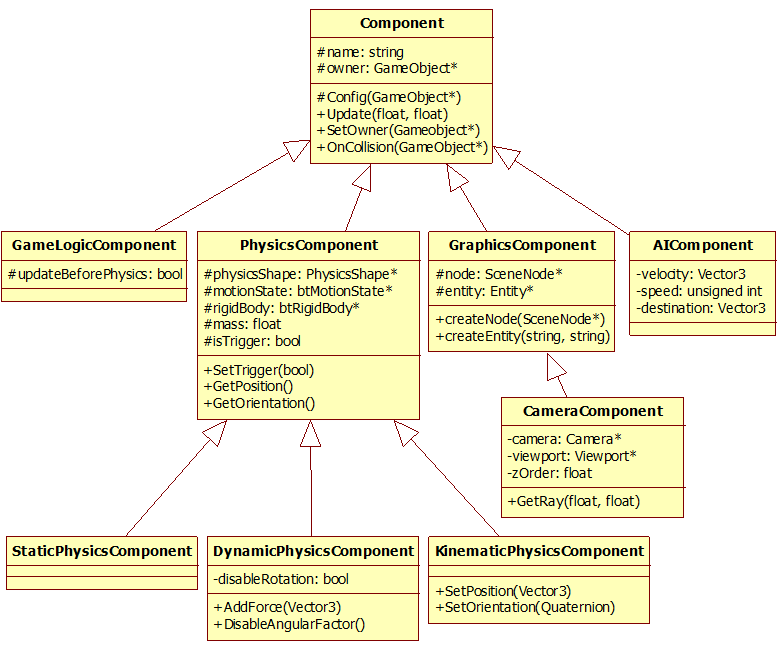
\includegraphics[width=110mm, keepaspectratio]{figures/old_engine_components.png}
\caption{Szakdolgozatom motor oldali komponenseinek UML oszt�lydiagrammja}
\label{fig:BScThesisEngineComponents}
\end{figure}

\begin{figure}[!ht]
\centering
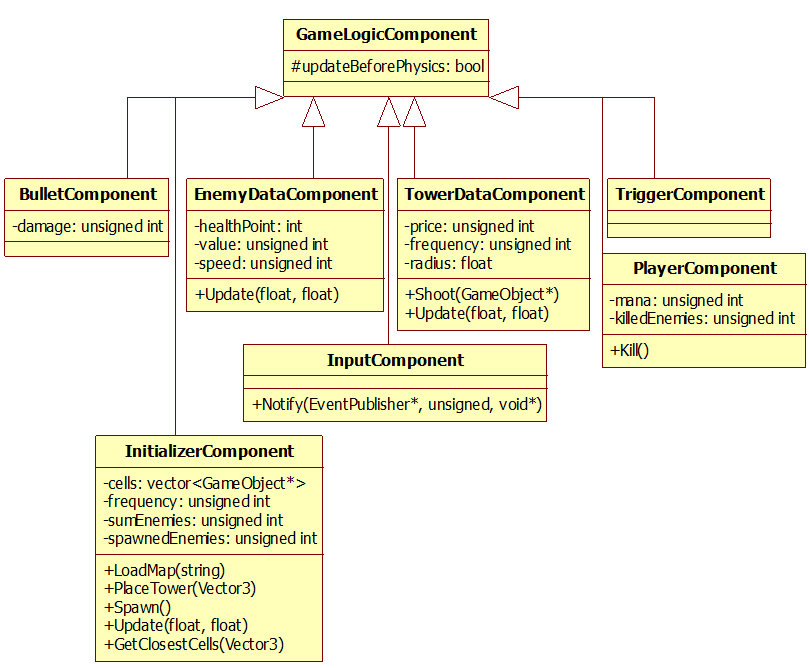
\includegraphics[width=110mm, keepaspectratio]{figures/old_game_components.png}
\caption{Szakdolgozatom j�t�klogika oldali komponenseinek UML oszt�lydiagrammja}
\label{fig:BScThesisGameComponents}
\end{figure}

A mesterk�pz�s kezdeti szakasz�ban megsz�ntettem a komponensek
redund�ns t�rol�s�t, melyet az okozott, hogy a j�t�kobjektumokban is �s a megfelel� alrendszerekben
is el voltak t�rolva a komponensek. Emiatt v�ltozott a komponensek befriss�t�si mechanizmusa is,
aminek a l�nyege, hogy a befriss�t�si sorrend meghat�roz�s�hoz a megfelel� befriss�t�si f�ggv�nyeket
kell a komponenseknek fel�ldefini�lniuk, melyek megh�v�s�r�l a gazda \textit{GameObject} gondoskodott.
�j funkcionalit�sok implement�l�s�val is foglalkoztam, ugyanis ebben az id�szakban val�s�tottam meg
egy alap hang alrendszert, melyet az OpenAL felhaszn�l�s�val val�s�tottam meg. Emellett megval�s�tottam
a virtu�lis vil�g XML-b�l t�rt�n� bet�lt�s�t is, melynek k�sz�nhet�en a kor�bbiakn�l egyszer�bben tudtam
le�rni a bet�ltend� sz�nteret, illetve annak m�dos�t�sa eset�n ennek k�sz�nhet�en m�r nem kellett t�bb�
�jraford�tanom a k�dot, ami a fejleszt�s felgyors�t�s�t is eredm�nyezte. Szint�n erre az id�szakra
tehet� a f�nyforr�sok beemel�se motor oldalra, illetve az OGRE overlay elemeinek alapszint�,
j�t�klogika oldali felhaszn�l�sa is.

A diplomaterv sor�n az eddigre kialakult rendszert k�v�nom tov�bbfejleszteni az el�z� szakaszban
le�rtaknak megfelel�en.

A legf�bb c�lom ezzel a diplomatervvel egy olyan eszk�z l�trehoz�sa, mely a k�s�bbiekben alapot
szolg�ltathat m�s dolgozatok elk�sz�t�s�hez illetve esetlegesen oktat�si seg�danyagk�nt is
felhaszn�lhat� a k�s�bbiek folyam�n.

%----------------------------------------------------------------------------
\subsection{A komponens alap� megk�zel�t�s}
%----------------------------------------------------------------------------

%----------------------------------------------------------------------------
\subsubsection{�r�kl�s eset�n felmer�l� probl�m�k}
%----------------------------------------------------------------------------
K�pzelj�k el a k�vetkez�t: �r�kl�sen alap� rendszert akarunk l�trehozni, melynek alapja egy absztrakt
�soszt�ly, \textit{GameObject} n�ven. Ebb�l az �soszt�lyb�l �r�k�ltet�nk egy \textit{Dynamic} �s egy
\textit{Static} oszt�lyt, melyek a mozg� �s nem mozg� j�t�kobjektumokat reprezent�lj�k.
De ezek m�g mindig absztrakt oszt�lyok, vagyis nem lehet �ket p�ld�nyos�tani.
Ahhoz, hogy objektumokat kapjunk, tov�bbi lesz�rmaz�sokat kell tenn�nk. Legyen egy \textit{Dynamic}
lesz�rmazott \textit{Car} n�ven, illetve egy \textit{Static} lesz�rmazott \textit{House} n�ven.
Ezeken fel�l ha l�trehozunk egy \textit{Caravan} oszt�lyt, mely sz�rmazik a \textit{Car} �s a
\textit{House} oszt�lyb�l is, akkor m�ris fat�lis logikai hib�ba �tk�zt�nk, hiszen a \textit{Caravan}
az egyszerre \textit{Dynamic} �s \textit{Static} is, ami term�szetesen ellentmond�shoz vezet (\figref{BadInheritance} �bra).

\begin{figure}[!ht]
\centering
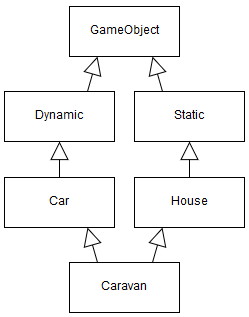
\includegraphics[width=40mm, keepaspectratio]{figures/bad_inheritance.png}
\caption{Ellentmond�s: a Caravan egyszerre Dynamic �s Static is} 
\label{fig:BadInheritance}
\end{figure}

Az olvas� gondolataiban persze jogosan megfogalmaz�dhat, hogy ezt az egyszer� rendszert
le lehetne cser�lni egy olyanra, ahol probl�mamentesen megf�rne egym�s mellet az aut�, a h�z illetve
a lak�kocsi oszt�ly is. Ez �gy is van, de a gyakorlatban nem h�rom, hanem sokkal t�bb j�t�kobjektummal
kell dolgozniuk a programoz�knak, s egy hatalmas �r�kl�si rendszerbe besz�rni egy �jabb t�pus�
j�t�kobjektumot sokszor vezethet hasonl� anom�li�khoz, mint amilyet az el�bbiekben ismertettem.

Ezek ut�n m�r tal�n nem is olyan meglep�, hogy az iparban manaps�g nem az �r�kl�sen alapul� rendszereket
r�szes�tik el�nyben. A tov�bbiakban egy alternat�v megk�zel�t�st ismertetek.

%----------------------------------------------------------------------------
\subsubsection{Lesz�rmaz�s helyett tartalmaz�s}
%----------------------------------------------------------------------------
Ebben a rendszerben kiz�r�lag egyetlen j�t�kobjektum oszt�ly van, illetve ezen k�v�l vannak komponensek
is. Minden komponens egyetlen j�l meghat�rozott funkcionalit�s�rt felel, p�ld�ul a kirajzol�s�rt, a
fizik��rt, stb. �ltal�ban ilyen rendszerek eset�n a felhaszn�l�nak is lehet�s�ge van �j komponensek
l�trehoz�s�ra.

A m�dszer l�nyege, hogy a j�t�kobjektum tulajdons�gait kiz�r�lag az hat�rozza meg, hogy milyen t�pus�
komponensek vannak hozz�rendelve, vagyis a j�t�kobjektumt�l elcsatoljuk annak tulajdons�gait (\figref{ComponentBased} �bra).
Ez egyszerre lehet �ld�s �s �tok is. �ld�s, hiszen egy ilyen rendszer sokkal rugalmasabb �s karbantarthat�bb lehet,
mint az �r�kl�sen alapul� megold�s (gondoljunk csak arra, hogy az objektumok tulajdons�gait dinamikusan,
fut�s k�zben is nagyon egyszer�en m�dos�thatjuk), emellett viszont �tok is egyben, hiszen egy ilyen rendszer
megval�s�t�s�hoz el kell vonatkoztatnunk att�l az objektumorient�lt szeml�letm�dt�l, amiben
egy�bk�nt a programoz�k jelent�s h�nyada k�pes gondolkodni.

\begin{figure}[!ht]
\centering
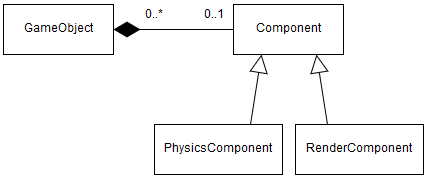
\includegraphics[width=70mm, keepaspectratio]{figures/component_based.png}
\caption{Funkcionalit�s elcsatol�sa az objektumt�l}
\label{fig:ComponentBased}
\end{figure}

Ennek a m�dszernek a seg�ts�g�vel az el�z� szakaszban felvetett probl�m�t egyszer�en meg lehet oldani.
Ehhez l�tre kell hozni h�rom \textit{GameObject} p�ld�nyt a megfelel� komponensekkel. A \textit{Car}
objektumhoz a \textit{WheelComponent} komponenst, a \textit{House} objektumhoz a \textit{KitchenComponent}
komponenst illetve a \textit{Caravan} objektumhoz mindk�t el�bb eml�tett komponenst
hozz�rendelj�k (\figref{SolutionWithComponents} �bra).

\begin{figure}[!ht]
\centering
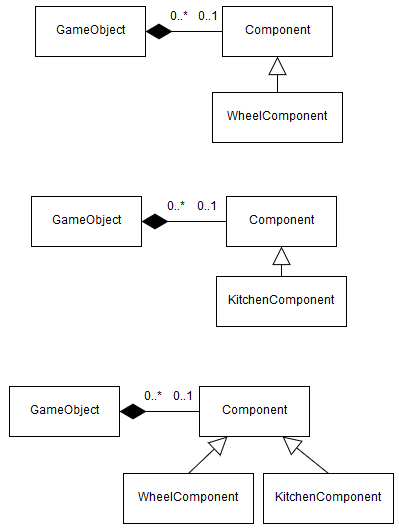
\includegraphics[width=60mm, keepaspectratio]{figures/all_compbased.png}
\caption{A feladat megold�sa komponensekkel}
\label{fig:SolutionWithComponents}
\end{figure}

%----------------------------------------------------------------------------
\subsection{3rdparty alrendszerek}
\label{subsec:3rdparty}
%----------------------------------------------------------------------------
Term�szetesen nem volt -- �s nem is lehetett -- c�lja a szakdolgozatomnak, hogy minden egyes
funkcionalit�st saj�t magam implement�ljak, hiszen ennek a v�ghez vitele t�lmutatott volna a
tant�rgy terjedelmi �s id�korl�tain. Ennek megfelel�en a fontosabb r�szfeladatokhoz m�r meglev�,
ingyenes �s platform-f�ggetlen eszk�z�ket haszn�ltam fel, melyeket a tov�bbiakban ismertetek.
%----------------------------------------------------------------------------
\subsubsection{OGRE 3D}
%----------------------------------------------------------------------------
A j�t�kmotorok egyik legalapvet�bb funkcionalit�sa a virtu�lis vil�g megjelen�t�s�nek k�pess�ge.
Ennek megval�s�t�s�hoz k�l�nf�le grafikai alrendszereket haszn�lnak fel, melyek lehetnek a motort�l
teljesen k�l�n v�l� k�ls� k�nyvt�rak, vagy �ppen a motorhoz fejlesztett bels� eszk�z�k is. Az �n
megval�s�t�somban nem volt c�l egy ilyen bels� eszk�z megval�s�t�sa, �gy egy erre a c�lra alkalmas
k�ls� k�nyvt�rat, az OGRE-t haszn�ltam fel, melyet az al�bbiakban ismertetek.

Az OGRE (\textbf{O}bject-Oriented \textbf{G}raphics \textbf{R}endering \textbf{E}ngine), vagyis
az objektumorient�lt grafikai megjelen�t� motor egy sz�nt�r alap�, rugalmas 3D grafikai motor,
melyet C++ nyelven k�sz�tettek\cite{OGRE}. C�lja, hogy k�nnyebb� tegye a fejleszt�k sz�m�ra olyan
alkalmaz�sok k�sz�t�s�t, melyek hardveresen gyors�tott grafikai megjelen�t�seket is ig�nybe vehetnek.
Ez a k�nyvt�r elvonatkoztat az alatta lev� grafikai k�nyvt�rakt�l (mint p�ld�ul DirectX, OpenGL),
s ezek haszn�lat�hoz biztos�t egy egys�ges interf�szt a szoftverrendszer t�bbi szerepl�je sz�m�ra.

J�n�h�ny grafikai motorral ellent�tben tervez�s-orient�lt, s nem funkci�-orient�lt m�don k�sz�lt,
vagyis a fejleszt�s sor�n a letisztult szoftver-strukt�ra legal�bb olyan fontos volt, mint a
megval�s�tott funkci�k mennyis�ge. Ennek k�sz�nhet�en kell�en �ltal�nos lett ahhoz, hogy b�rmilyen
t�pus� j�t�k elk�sz�t�s�hez megfelel�en alkalmazhat� legyen. Ezek mellett a meglehet�sen gazdag
dokument�ci�ja is hozz�j�rult ahhoz, hogy ilyen m�rt�kben elterjedjen a j�t�kfejleszt�k k�r�ben.

Elterjedts�g�nek ellen�re azonban az OGRE n�pszer�s�ge folyamatosan cs�kken. Ez t�bbek k�z�tt
betudhat� annak, hogy a fejleszt�i k�z�ss�g az ut�bbi id�ben nem mutatott megfelel� aktivit�st
(a Visual Studio 2015-h�z ford�tott 1.9-es SDK 2016 december�ben jelent meg, s azt is csak egy
f�rumoz� kommentj�ben lehetett megtal�lni), illetve magyar�zhat� azzal a tendenci�val is, hogy
manaps�g a j�t�kfejleszt�k el�nyben r�szes�tik azokat a szoftver-rendszereket, melyek nem csak a
megjelen�t�s�rt, hanem m�s funkcionalit�sok elv�gz�s��rt is felel�sek. Ez azonban nem kiz�r�lag az
OGRE probl�m�ja, hiszen �ltal�noss�gban elmondhat�, hogy az �ltal�nos c�l� j�t�kmotorok kezdik
kiszor�tnani a piacr�l a funkci�-specifikus motorokat.
%----------------------------------------------------------------------------
\subsubsection{OIS}
%----------------------------------------------------------------------------
Az OIS (\textbf{O}bject \textbf{O}riented \textbf{I}nput \textbf{S}ystem) platformf�ggetlen C++
oszt�lyk�nyvt�r, melynek feladata a k�l�nb�z� felhaszn�l�i bemenetek kezel�se.
Az OGRE az 1.4-es verzi�ja �ta haszn�lja\cite{OIS}.

%----------------------------------------------------------------------------
\subsubsection{Boost}
%----------------------------------------------------------------------------
A Boost C++ szabv�nyon alapul� modern k�nyvt�rak gy�jtem�nye. Ny�lt forr�sk�d�, platformf�ggetlen projekt,
mely a legt�bb n�pszer� C++ ford�t�t t�mogatja\cite{Boost}.

%----------------------------------------------------------------------------
\subsubsection{Bullet}
%----------------------------------------------------------------------------
A virtu�lis vil�g megjelen�t�se csak a legritk�bb esetben elegend� egy grafikus alkalmaz�s -- 
p�ld�ul egy sz�m�t�g�pes j�t�k -- elk�sz�t�s�hez. Manaps�g szinte k�telez� eleme a j�t�kmotoroknak
valamilyen fizikai motor, mely a programoz�k �ltal felparam�terezett fizikai vil�g viselked�s�t k�pes
szimul�lni \textemdash{} bizonyos keretek k�z�tt --- val�s id�ben.

Az ilyen alrendszerek elk�sz�t�se k�zel sem trivi�lis feladat, �gy lev�ve ezt a terhet a
j�t�klogika-programoz�k v�ll�r�l az �n motorom is tartalmaz fizikai alrendszert, melynek megval�s�t�s�hoz
a Bullet nev� fizikai motort haszn�ltam fel\cite{Bullet}.

A Bullet ingyenes, platform f�ggetlen, ny�lt forr�sk�d� fizikai motor. F�bb funkci�i k�z�tt megeml�tend�
a merev- �s puhatest szimul�ci� illetve a diszkr�t �s folytonos �tk�z�s-detekt�l�s. Jelenlegi legfrissebb
stabil verzi�ja a 2.87-es.

Ami a piaci alkalmaz�s�t illeti, a sz�m�t�g�pes j�t�kok ter�let�n ezt a szoftvert haszn�lt�k fizikai
szimul�ci�khoz a Rockstar Games sz�mos alkot�s�n�l (GTA IV, GTA V, Red Dead Redemption), az
Activision c�g Blood Drive nevezet� j�t�k�n�l, vagy �ppen a DIRT sorozat �sszes r�sz�n�l.
Sz�mos hollywood-i alkot�s is alkalmazta m�r a Bullet-et merev testek fizikai szimul�ci�in�l a
speci�lis effektek megalkot�s�hoz. P�ldak�nt megeml�thet� a Shrek 4 a PDI/Dreamworks-t�l, vagy a
Framestore 2009-es k�zrem�k�d�s�vel l�trej�tt Sherlock Holmes film.

%----------------------------------------------------------------------------
\subsubsection{TinyXML}
%----------------------------------------------------------------------------
C++-ban �rt, platformf�ggetlen, ny�lt forr�sk�d�, ingyenes XML feldolgoz�\cite{TinyXML}.

%----------------------------------------------------------------------------
\section{Diplomaterv fel�p�t�se}
%----------------------------------------------------------------------------
A dolgozat m�sodik fejezete az eddigi munk�m �tdolgoz�s�val foglalkozik, kit�rve az egyes m�dos�tand�
egys�gekre, �gy mint a projektek build-el�si folyamatai, az XML-feldolgoz� alrendszer, az er�forr�sok
kezel�se �s anyagok le�r�sa.

A dolgozat harmadik fejezete a diplomaterv legl�nyegesebb r�sze, ugyanis ebben a fejezetben foglalkozok
a komponens alap� motorom b�v�t�s�vel. Ebben a fejezetben kit�rek az �sszes olyan pontra, melyek
a feladatki�r�sban szerepelnek, majd a fejezetet egy �ttekint� szakasszal z�rom.

A dolgozat negyedik fejezete arra szolg�l, hogy bizony�tsa az elk�sz�lt motor m�k�d�k�pess�g�t egy
demonstr�ci�s alkalmaz�son kereszt�l. Ebben a fejezetben ismertetem a demonstr�ci�s alkalmaz�s fel�
t�masztott k�vetelm�nyeket, az alkalmaz�s megval�s�t�s�nak menet�t, majd egy �ttekint� szakasz ut�n
az alkalmaz�s tesztel�s�vel z�rom a fejezetet.

A dolgozat �t�dik fejezete az elk�sz�lt programok �rt�kel�s�vel foglalkozik, mely haszn�lhat�s�g,
k�dmin�s�g �s sebess�g szempontj�b�l vizsg�lja meg a dolgozat eredm�nyek�nt l�trej�tt szoftvereket.

V�g�l a dolgozat �sszefoglal�ssal �s kitekint�ssel z�rul a hatodik fejezetben.

%----------------------------------------------------------------------------
\chapter{A keretrendszer �tdolgoz�sa}
%----------------------------------------------------------------------------
Az al�bbi fejezet bemutatja azokat a m�dszereket, melyek seg�ts�g�vel m�dos�tottam a szoftverk�rnyezet
fel�p�t�s�t annak �rdek�ben, hogy annak build-el�si m�dja, karbantarthat�s�ga illetve b�v�thet�s�ge
javuljon a kor�bbi rendszerhez k�pest.

%----------------------------------------------------------------------------
\section{Projektek build-el�se}
%----------------------------------------------------------------------------

%----------------------------------------------------------------------------
\subsection{Build-el�si id� cs�kkent�se}
%----------------------------------------------------------------------------
C++ projektek eset�ben nem lehet figyelmen k�v�l hagyni a build-el�si id� hossz�t, hiszen ez az
egyik leglassabban build-el� programoz�si nyelv, ami a komplexit�s�b�l ad�dik. Kor�bbi munk�im
sor�n nem t�r�dtem ezzel a metrik�val, hiszen a projektek m�rete �s bonyolults�ga miatt az
�jrabuild-el�sek ideje sem volt sz�mottev�, viszont a szakdolgozatom eredm�nyek�nt megsz�letett
szoftverre ezt nem lehetett elmondani. A fejleszt�si id� v�ge fel� kifejezetten hossz� ideig tartott
egy-egy kisebb m�dos�t�s ut�ni build-el�s ideje is, ez�rt hat�roztam el azt, hogy id�met �s energi�mat
nem sajn�lva megpr�b�lom cs�kkenteni a build-el�si folyamat idej�t, hiszen ha ezt nem tenn�m meg, akkor
a k�s�bbi -- feltehet�leg nagyobb -- k�db�zis eset�n a v�rakoz�si id�k m�g hosszabbak lenn�nek.

Az legfontosabb k�vetend� elv volt sz�momra a header f�jlok szerep�nek cs�kkent�se. Ez azt
jelenti, hogy minimaliz�lni kell az \verb+#include+-okat illetve a f�ggv�ny defin�ci�kat ezekben
a f�jlokban. Mindez az�rt hasznos, mert �gy cs�kkenthet� a header f�jlok v�ltoz�si gyakoris�ga, �gy
ritk�bban kell azokat illetve az azokat haszn�l� f�jlokat �jraford�tani. Teh�t egy source f�jlban
t�rt�n� v�ltoz�s sokkal ``olcs�bb'', mint egy header-beli v�ltoz�s, mivel a source f�jlt nem 
\verb+#include+-olja senki, �gy a v�ltoz�sa nem �rint m�s f�jlokat.

A header f�jlokban lev� \verb+#include+-ok sz�m�nak minimaliz�l�s�ra egy bev�lt m�dszer az el�deklar�l�s
m�dszere. Ennek az a l�nyege, hogy ha egy header f�jlban haszn�lok egy szimb�lum nevet (pl.: egy oszt�ly
neve), viszont nem haszn�lom annak defin�ci�j�t (pl.: egy oszt�ly tagf�ggv�ny�t), akkor igaz�b�l
abban a f�jlban nincs is sz�ks�g a haszn�lt szimb�lum defin�ci�j�ra, csak a nev�nek el�deklar�l�s�ra.
Ebben az esetben a t�nyleges defin�ci� haszn�lata -- teh�t a t�nyleges \verb+#include+-ol�s -- a source
f�jlban t�rt�nik meg. Megjegyzend�, hogy ez a m�dszer hat�konyan haszn�lhat� a k�rk�r�s dependenci�k
probl�m�j�nak felold�s�ra is. Mindezeken t�l a dependenci�k sz�m�nak kord�ban tart�s�ra is megfelel�
m�dszer az \verb+#include+-ok sz�m�nak minimaliz�l�sa, hiszen gondoljunk csak bele, ha egy header
f�jlt valamely k�dr�szbe beemelek, akkor nem csak annak a tartalma, hanem az � \verb+#include+
f�jljainak a tartalma is beemel�dik, �s �gy tov�bb, tranzit�v m�don. �gy k�nnyen el�fordulhat, hogy
a t�nylegesen beemelt k�dmennyis�gnek csak a t�red�k�t szeretn�nk t�nylegesen haszn�lni.

\begin{lstlisting}[frame=single,float=!ht,
caption={P�lda el�deklar�l�sra a C++ nyelvben}, label=ForwardDeclarationCpp]
// forward declaration of class A
class A;
class B
{
	A* pA;	// there is no need for the definition of class A
};
\end{lstlisting}

Egy m�sik technika is a header f�jlokhoz k�thet�, miszerint haszn�ljunk include guard-okat. Ennek
a techik�nak a l�nyege, hogy a header tartalm�t a compiler csak akkor parszolja be, ha azt m�g nem
tette meg. Ezt header f�jlonk�nt k�l�n makr�k defini�l�s�val tehetj�k meg. Modernebb ford�t�k t�bbs�ge
t�mogatja a \verb+#pragma once+ preprocesszor direkt�v�t is (annak ellen�re, hogy ez nem a szabv�ny r�sze),
melynek haszn�lat�val ugyan azt az eredm�nyt lehet el�rni, mint az include guard-os makr�k defini�l�s�val.
Az �n k�djaimban a k�t ismertetett megold�st egy�tt haszn�lom, �gy a k�v�nt funkcionalit�st olyan
ford�t�k eset�n is el tudom �rni, melyek nem t�mogatj�k a \verb+#pragma once+ haszn�lat�t.

\begin{lstlisting}[frame=single,float=!ht,
caption={Include guard �s pragma once egy�ttes haszn�lata}, label=IncludeGuardsCpp]
#ifndef INCLUDE_GUARD
#define INCLUDE_GUARD

#pragma once

/* header content goes here */

#endif
\end{lstlisting}

Az im�nt eml�tett m�dszerek mellett n�pszer� megold�s az el�ford�tott header f�jlok haszn�lata is.
Ennek a technik�nak az a l�nyege, hogy l�trehozunk egy olyan header f�jlt, melyben az olyan
\verb+#include+-ol�sok szerepelnek, melyek nagy m�ret�ek, sok helyen kell haszn�lni �ket illetve
soha -- vagy csak nagyon ritk�n -- v�ltoznak. Ennek a f�jlnak a l�trehoz�sa ut�n megmondhatjuk
a kurrens ford�t�nak -- ha az t�mogatja --, hogy kezelje ezt a header f�jlt el�ford�tottk�nt, vagyis
ezt ford�tsa le els�nek, �s egyetlen egyszer, s linkel�skor a m�r meglev� object f�jlt kelljen
haszn�lni. Ez is tipikusan egy olyan m�dszer, mellyel esetenk�nt t�bbsz�r�s gyorsul�st lehet
el�rni az eredeti build-el�si m�dszerhez k�pest, viszont ha nem megfelel�en haszn�lj�k, akkor
ak�r t�bbet is �rthat, mint haszn�lhat.

A felsorolt m�dszereken k�v�l term�szetesen m�g sz�mos m�s technika is l�tezik a C++-os projektek
build-el�si idej�nek cs�kkent�s�re, s a lista val�sz�n�leg a j�v�ben m�g tov�bb fog gyarapodni, hiszen
az gyors�t�sra val� ig�ny tov�bbra is megvan a fejleszt�k k�r�ben.
%----------------------------------------------------------------------------
\subsection{Bin�risok m�reteinek cs�kkent�se}
%----------------------------------------------------------------------------
Mint ahogy arr�l kor�bban m�r �rtam, a motort egy dinamikus k�nyvt�rba ford�tom bele.
Ahhoz, hogy az egyes motorban implement�lt funkcionalit�sok a j�t�klogika oldal�n is el�rhet�ek legyenek,
explicite meg kell mondani a ford�t�programnak, hogy azt tegye el�rhet�v� a k�nyvt�rt haszn�l�k sz�m�ra.
Ezt gyakran �gy szokt�k megoldani, hogy ha egy oszt�lynak egy adott f�ggv�ny�re sz�ks�g van a k�nyvt�ron
k�v�l is, akkor az eg�sz oszt�ly kiker�l a k�nyvt�r publikus interf�sz�re. Ez gyakran nem t�l szerencs�s,
ugyanis legt�bbsz�r ezzel a megold�ssal sok olyan dolgot is kiaj�nlunk a k�nyvt�r haszn�l�i sz�m�ra,
melyekre igaz�b�l nincs is sz�ks�g�k. Ezzel a megk�zel�t�ssel �ppen ez�rt indokolatlanul nagyra
lehet n�velni a k�nyvt�r m�ret�t.

Ennek a probl�m�nak a megold�s�ra minimaliz�ltam a k�nyvt�rba beker�l� tartalmat, melynek hat�s�ra
a motor m�rete 3.35MB-r�l 3.29MB-ra, a j�t�k m�rete 475KB-r�l 290 KB-ra cs�kkent.

Ezek mellett kijav�tottam egy r�g�ta elh�z�d� hib�t, melynek az volt a kiv�lt� oka, hogy a Bullet-hez
-- figyelmetlens�gem miatt -- statikusan linkeltem a C Runtime-ot, melynek k�vetkezt�ben a motoromn�l
is r� voltam k�nyszer�lve a statikus linkel�sre a linker error-ok elker�l�se v�gett. A p�ldaj�t�k viszont
tov�bbra is dinamikusan linkelte mag�hoz a C Runtime-ot, aminek k�vetkezt�ben el�fordulhattak olyan
esetek dinamikus mem�riafoglal�sn�l, mikor pl. a motor oldalon foglalom le a mem�ri�t, de a j�t�k oldalon
pr�b�lom felszabad�tani, ami a legjobb esetben is assert-et okoz, mivel a j�t�k egy olyan mem�riater�letet
akar felszabad�tani, amit nem is l�t, mivel m�sik heap-en lett foglalva.

Ezt -- miut�n r�j�ttem a hiba forr�s�ra -- m�r trivi�lis volt kijav�tani, hiszen csak a megfelel�
Bullet-hez tartoz� statikus k�nyvt�rakat kellett �jraford�tani �gy, hogy dinamikusan linkelj�k
magukhoz a C Runtime-ot, majd az engine-re is alkalmazva ezt a be�ll�t�st a fentebb eml�tett
probl�m�k megsz�ntek. A jav�t�s ut�n az engine m�rete -- mivel m�r nem tartalmazta mag�ban a
C Runtime-ot -- lecs�kkent 1.8MB-ra.

%----------------------------------------------------------------------------
\subsection{CMake haszn�lata}
%----------------------------------------------------------------------------
Az automatiz�lt build-el�s a szoftverfejleszt�s egyik fontos folyamata, melynek k�sz�nhet�en az
alkalmaz�s elk�sz�t�s�t minden egyes alkalommal ugyanazokkal a l�p�sekkel, be�ll�t�sokkal illetve
param�terekkel lehet megtenni. A k�db�zis n�veked�s�vel egyre nagyobb ig�ny van az ilyen eszk�z�k
haszn�lat�ra.

Egy ilyen eszk�z a CMake is, ami egy olyan ny�lt forr�s� rendszer, mely platform- �s ford�t�f�ggetlen
m�don kezeli a futtathat� �llom�nyok l�trehoz�si folyamatait. A legt�bb platformf�ggetlen rendszerrel
ellent�tben a CMake nem k�n�l saj�t �p�t�si folyamatot, hanem az aktu�lis platform nat�v k�rnyezet�t
haszn�lja erre a c�lra. 


ide kell minden a cmake-rol

h�tha m�s platformon is m�k�dne a programom

a visual studio be�ll�t�sai k�z�tt matatni sem le�ny�lom + k�nny� elrontani
nagy projektekn�l ez egyszer�bb, mint mindig k�zzel be�ll�tani a dependenci�kat a user-ekn�l

a visual studio nem szemeteli tele a forras konyvtarakat

A projekt k�nyvt�rszerkezet�nek kialak�t�sa

%----------------------------------------------------------------------------
\section{Jelenetek kezel�se}
%----------------------------------------------------------------------------
A szakdolgozatom sor�n implement�lt megold�sban a jelenet le�r�sa kiz�r�lag a p�lya le�r�s�ra korl�toz�dott
(teh�t p�ld�ul j�t�kobjektumok kezdeti transzform�ci�it nem lehetett benne le�rni),
r�ad�sul azt is csak k�t dimenzi�s s�kk�nt lehetett �rtelmezni, ennek megfelel�en b�rmely le�r� f�jl
k�t dimenzi�s koordin�t�kat tartalmazott (x, illetve z koordin�t�k).

Term�szetesen ez a megold�s egyr�szt er�sen korl�tozza a felhaszn�l� szabads�g�t a kialak�that� jelenet
milyens�g�ben (p�ld�ul a p�lya talaja nem lehet tetsz�leges domborzat, mindenk�pp s�knak kell lennie),
m�sr�szt �sszetettebb le�r�sok k�sz�t�se f�rads�gos munka, r�ad�sul ha az eredm�ny nem
felel meg az elv�r�soknak, akkor el�g neh�z �szrevenni a hiba ok�t egy hosszadalmas le�r�sban.

Jelen diplomatervez�s sor�n az el�z�t�l teljesen k�l�nb�z� megold�st implement�ltam, melynek seg�ts�g�vel
a felhaszn�l�nak lehet�s�ge ny�lik bonyolultabb jelenetek le�r�s�ra is.

Ehhez defini�ltam egy olyan XML form�tumot, mely illeszkedik ahhoz a komponens alap� szeml�lethez,
melyet az eg�sz rendszer k�pvisel. Ez azt jelenti, hogy az XML le�r�s j�t�kobjektumok le�r�sainak az
�sszess�ge, amely le�r�sok pedig komponensek le�r�saib�l tev�dnek �ssze. Az XML form�tum ismertet�s�t
a F�ggel�k tartalmazza.

Ennek megfelel�en a megval�s�t�s sor�n komponens parszereket kellett k�sz�tenem,
melyek �ltal l�trehozott komponenseket a sz�l� XML-tag �ltal reprezent�lt j�t�kobjektumokhoz kell hozz�f�zni.
�gy a jelenetle�r� XML f�jl egyetlen rekurz�v top-down bej�r�s�val a felhaszn�l� �ltal le�rt jelenet
 -- a megfelel� komponens parszerek megl�t�ben -- megjelenik a szimul�ci� kezdet�n.
Onnant�l kezdve a fizikai vil�g szab�lyai illetve a felhaszn�l�i esem�nyek induk�lhatj�k a virtu�lis
vil�g v�ltoz�sait.

Az XML parszol�s�hoz a TinyXML nev� eszk�zt haszn�ltam fel, amely egy C++-ban �rt, platformf�ggetlen,
ny�lt forr�sk�d�, ingyenes XML feldolgoz� k�nyvt�r.

%----------------------------------------------------------------------------
\section{Bemenetek kezel�se}
%----------------------------------------------------------------------------
Ezel�tt a bemeneti eszk�z�k esem�nyeit kiz�r�lag pollingol�s m�dszerrel figyeltem, ami azt jelenti,
hogy minden frame-ben r� kellett n�znem a bemeneti eszk�z�k aktu�lis �llapotaira. Ennek a megold�snak
az az el�nye, hogy mindig pontosan tudom, hogy az update-el�si l�nc melyik r�sz�r�l polling-olok.
A megold�snak a h�tr�nya viszont az, hogy nem k�lts�g-hat�kony, hiszen a frame-enk�nti ellen�rz�s
t�l sok f�l�sleges kommunik�ci�t vihet a rendszerbe.

Ezt a megold�st kieg�sz�tettem azzal, hogy a bemeneti esem�nyeket figyel� oszt�lyom (InputManager)
feliratkozik OIS esem�nyekre, s mint ahogy azt az Observer tervez�si mint�n�l megszokhattuk, b�rmilyen
bemeneti eszk�z-esem�nyr�l �rtes�t�st kap, s megh�v�dik a megfelel� esem�nykezel� f�ggv�nye. Ennek a
megold�snak az az el�nye, hogy az esem�nykezel� k�d kiz�r�lag akkor h�v�dik meg, amikor az esem�ny
bek�vetkezett, teh�t nincs f�l�sleges kommunik�ci�s overhead. A megold�s h�tr�nyak�nt ugyanakkor
megeml�thet�, hogy nem tudjuk azt, hogy az esem�nykezel� f�ggv�ny az update-l�nc melyik szakasz�ban
h�v�dott meg.

Ahogy l�that�, mindk�t megold�snak megvannak az el�nyei illetve a h�tr�nyai egyar�nt, �ppen ez�rt
a felhaszn�l� d�nthet arr�l, hogy mikor melyik m�dszert k�v�nja haszn�lni a bemeneti esem�nyek
kezel�s�re.

%----------------------------------------------------------------------------
\section{Transzform�ci�k kezel�se}
%----------------------------------------------------------------------------
A szakdolgozatomban a j�t�kobjektumok tagv�ltoz�k�nt tartalmazt�k a kurrens poz�ci�jukat illetve
orient�ci�jukat, ennek megfelel�en k�l�n�ll�, transzform�ci�k�rt felel�s komponens m�g nem l�tezett
a rendszerben akkoriban.
Ez az�rt nem volt el�ny�s, mert a rendszer b�v�t�si �tletei k�z�tt szerepelt a
j�t�kobjektumok hierarchi�ba t�rt�n� rendez�s�nek k�pess�ge, aminek �gy a megval�s�t�sa is a
j�t�kobjektumokat reprezent�l� oszt�lyba ker�lt volna elhelyez�sre, t�ls�gosan megn�velve annak m�ret�t,
illetve megnehez�tve annak kezel�s�t.

Ennek a probl�m�nak a kik�sz�b�l�s�re hoztam l�tre a rendszeremben a geometriai transzform�ci�k�rt
(eltol�s, forgat�s illetve sk�l�z�s) felel�s motor oldali komponenst, a TransformComponent-et.
A rendszeremben ez az egyik legfontosabb komponens t�pus, ugyanis ez az egyetlen olyan komponens-
lesz�rmazott, melyet alap�rtelmezetten hozz�rendelek minden j�t�kobjektumhoz. Emellett term�szetesen
rengeteg m�s komponens is t�maszkodik a transzform�ci�s komponens k�l�nb�z� funkcionalit�s�ra, �gy
nyugodtan kijelenthetem, hogy a motorom egyik alappill�r�t k�pezi ez az oszt�ly, helyes �s hat�kony
m�k�d�se teh�t kulcsk�rd�s a rendszer eg�sze szempontj�b�l. El�g, ha csak arra gondolunk, hogy a
j�t�kobjektumok hierarchi�kba rendez�dhetnek, �gy a gyerek j�t�kobjektumnak �r�k�lnie kell a sz�l�
j�t�kobjektumnak a transzform�ci�it (eltol�s, forgat�s, sk�l�z�s), illetve ha a felhaszn�l� egy
gyerek j�t�kobjektumnak a transzform�ci�it k�v�nja megadni, akkor azt a sz�l� j�t�kobjektum koordin�ta-
rendszer�ben kell megtennie.

Viszont amilyen fontos ennek az oszt�lynak a helyes �s hat�kony m�k�d�se, annyira nem trivi�lis ennek
az �llapotnak az el�id�z�se, ugyanis ehhez n�lk�l�zhetetlenek matematikai -- f�leg line�ris algebrai --
alapismeretek.

A megval�s�t�shoz a TransformComponent ny�lv�n tartja a hozz� tartoz� j�t�kobjektum transzform�ci�s
adatait (eltol�st, forgat�st, sk�l�z�st illetve az ezeket egys�gben reprezent�lni k�pes transzform�ci�s m�trixot) mind vil�gt�rben, mind a sz�l� koordin�ta-rendszer�ben. B�rmilyen m�dos�t�s hat�s�ra be kell
friss�teni az �sszes vektort/kvaterni�t/m�trixot a konzisztens �llapot �rdek�ben. A sok tagv�ltoz� miatt
az oszt�ly getter f�ggv�nyeinek k�lts�ge elhanyagolhat�, viszont az el�bb eml�tett konzisztens
�llapot megtart�sa miatt a setter f�ggv�nyek k�lts�ge nagys�grendekkel nagyobb, de ez �sszess�g�ben
nem volt zavar� t�nyez� a fejleszt�s �s a tesztel�s sor�n sem. Egy�bk�nt is a helyes m�k�d�st ez a
diplomaterv fontosabbnak tartja, mint a vill�mgyors m�k�d�st.

%----------------------------------------------------------------------------
\section{Er�forr�sok kezel�se}
%----------------------------------------------------------------------------
Kor�bban nem ford�tottam kell� figyelmet az er�forr�sok kezel�s�re, hiszen l�nyegtelen volt, hogy
milyen f�jlszerkezetben vannak elhelyezve, illetve milyen m�don vannak bet�ltve. Csak az sz�m�tott,
hogy a bet�lt�s sikeres legyen. Ezzel nem is volt gond addig, am�g a motor illetve a hozz� tartoz�
p�lda alkalmaz�s kis m�ret� volt, s kev�s er�forr�st haszn�lt.

Viszont ahogy n�tt a felhaszn�land� er�forr�sok sz�ma, �gy kezdett egyre neh�zkesebb� v�lni
a kezel�s�k. A rengeteg f�jl egyetlen mapp�ba s�r�tve �tl�thatatlann� tette azt, hogy mely
er�forr�sok tartoznak �ssze, s melyek nem. Tov�bb� azt sem volt trivi�lis kider�teni, hogy
mely er�forr�sok redund�nsak, vagy �ppen haszn�laton k�v�liek a p�lda alkalmaz�s �ltal.

A probl�m�k megold�s�ra a motor oldalon "be�getett" el�r�si �t helyett konfigur�ci�s f�jlokat kezdtem
el haszn�lni, s azokat beparszolni bet�lt�skor. Emellett az er�forr�sok t�rol�si m�dj�n is v�ltoztattam.
Ezel�tt az er�forr�sokat t�pusuk szerint t�roltam (a mesh-ek egy�tt, a text�r�k egy�tt, a materialok
egy�tt stb.), mostant�l viszont az er�forr�sokat objektumonk�nt t�rolom, ami azt jelenti, hogy egy
adott objektumhoz tartoz� f�jlok egy egys�gben foglalnak helyett, j�l elk�l�n�tve a t�bbi
er�forr�st�l.

Ennek a megold�snak tal�n a legnagyobb el�nye, hogy �j er�forr�sok illetve el�r�si utak felv�tele
ut�n a programot nem kell �jraford�tani (hiszen ett�l a konfigur�ci�s f�jl parszol�sa nem v�ltozik meg),
�gy jelent�s id�t lehet megtakar�tani. Emellett ha egy m�sik j�t�kban is haszn�lni szeretn�k egy
objektumot, akkor nem kell megkeresni a hozz� tartoz� er�forr�sokat a k�l�nb�z� almapp�kb�l,
teh�t ezzel a megold�ssal az er�forr�sok �jra felhaszn�lhat�ak m�s kontextusban is.
V�g�l, de nem utols� sorban mivel ezek az er�forr�sokb�l �ll� egys�gek t�m�r�tve foglalnak helyet a
sz�m�t�g�p h�tt�rt�r�n (.zip f�jlok), �gy t�rter�letet is lehet sp�rolni ezzel a megold�ssal.

resource group-okra bontas fajlrendszer szinten es a leiro fajlban is (minden resource group egy
jelenetnek feleltethet� meg)

%----------------------------------------------------------------------------
\section{Anyagjellemz�k le�r�sa}
%----------------------------------------------------------------------------
Egy j�t�kmotor lehet ak�rmennyire j�l haszn�lhat�, rugalmas �s hat�kony, ha nem tud grafikailag
elfogadhat� eredm�nyt produk�lni vele a felhaszn�l�, akkor igaz�b�l nem j� semmire.

Az OGRE-ben az anyagok le�r�s�ra material script-eket szok�s haszn�lni. Ezek olyan szkriptek, melyek
seg�ts�g�vel k�nnyen olvashat� form�ban lehet le�rni a legk�l�nf�l�bb anyagoktulajdons�gokat, illetve k�nyelmesen
lehet �rnyal�programoknak param�tereket �tadni. Pontosabban az anyagle�r� szkriptekben nem k�zvetlen�l
�rnyal�programokat, hanem azok egy OGRE-ben defini�lt absztrakci�it, az �gynevezett programokat
haszn�lhatjuk.

Az �rnyal�programok tekintet�ben csak az OpenGL j�hetett sz�ba, melynek �rnyal�nyelve a GLSL. Egy
alternat�va lehetett volna a DirectX is, de ennek haszn�lata akad�lyokba �tk�z�tt,
err�l r�szletesebben a \sectref{Engine} fejezetben �rok.

%----------------------------------------------------------------------------
\chapter{A j�t�kmotor b�v�t�se}
%----------------------------------------------------------------------------
Ez a fejezet tartalmazza a Bevezet� fejezetben ismertetett feladataimnak a megold�sait.

Els�k�nt bemutatja a j�t�kobjektumok k�sleltetett l�trehoz�s�nak megval�s�t�s�t, azt�n az
�llapotg�p alap� rendszerek taglal�s�t k�vet�en az anim�ci�s alrendszer �s a mesters�ges intelligencia
alrendszer implement�l�s�t ismerteti. Ezt k�vet�en r�szletezi a felhaszn�l�i fel�let l�trehoz�s�nak m�dj�t.
V�gezet�l a fejezet a -- m�r alapjaiben eddig is meglev� -- hangrendszer illetve r�szecskerendszer
tov�bbfejleszt�s�vel illetve az elk�sz�lt rendszer �ttekint�s�vel z�rul.

%----------------------------------------------------------------------------
\section{J�t�kobjektumok k�sleltetett l�trehoz�sa}
%----------------------------------------------------------------------------

%----------------------------------------------------------------------------
\subsection{Motiv�ci�}
%----------------------------------------------------------------------------
Kor�bban az XML parszol�s azt hat�rozta meg, hogy milyen legyen a bet�lt�tt virtu�lis vil�g a
kezdeti id�pontj�ban. Nem volt lehet�s�g olyan objektumok defini�l�s�ra, melyek p�ld�nyos�t�s�t
csak a virtu�lis vil�g egy k�s�bbi szakasz�ban lehetett volna v�ghez vinni.

Ig�ny viszont lett volna erre a funkcionalit�sra, gondoljunk csak egy l�fegyverre, mely valamilyen
l�ved�ket k�pes mag�b�l kibocs�tani egy adott esem�ny -- p�ld�ul bal eg�rgomb lenyom�sa -- hat�s�ra.
A l�ved�k le�r�s�nak term�szetesen helye van az XML le�r� f�jlban, m�gsem szeretn�nk, ha az azonnal
bet�lt�dne. Persze azt sem tudhatjuk, hogy h�ny p�ld�nyt defini�ljunk a le�r� f�jlban, mert ez
kiz�r�lag a felhaszn�l�t�l f�gg. Viszont azt sem szeretn�nk, ha minden l�ved�k-bet�lt�s el�tt az XML
f�jlhoz kellene fordulni, mert az nagyon lelass�tan� a program fut�s�t (a h�tt�rt�r el�r�si ideje
nagys�grendekkel nagyobb a mem�ria el�r�si idej�n�l).

M�sfel�l annak is van �rtelme, ha t�bb f�le l�ved�k t�pus l�tezik egy j�t�kban, s ezeknek vannak k�z�s
tulajdons�gaik. Ebben az esetben is hasznos lenne egy olyan absztrakt j�t�kobjektum defin�ci�
az XML le�r�sban, melyet k�zvetlen�l nem p�ld�nyos�tunk, viszont a tartalm�t felhaszn�lva
-- esetleg azt m�dos�tva -- konkr�t j�t�kobjektumokat lehet l�trehozni.

Ezen ig�nyek kiel�g�t�s�re tal�lt�k ki a prefab-okat, melyek implement�l�s�t a saj�t rendszeremben
az al�bbiakban ismertetek.

%----------------------------------------------------------------------------
\subsection{Megval�s�t�s}
%----------------------------------------------------------------------------
Mindezen funkcionalit�sok megval�s�t�s�ra lehet�v� tettem a motorom sz�m�ra a j�t�kobjektumok
k�sleltetett l�trehoz�s�t. A megval�s�t�snak a l�nyege, hogy minden komponenshez defini�lok egy-egy
le�r� strukt�r�t, mely tartalmazza az �sszes olyan param�tert, mely �tadhat� a hozz� tartoz�
komponensnek. A le�r� strukt�r�k mellett l�trehoztam egy \textit{GenericPrefab} nev� generikus oszt�lyt,
melynek feladata adott t�pus� l�trehoz� strukt�ra felt�lt�se �s alkalmaz�sa adott t�pus� komponensre.
A \textit{GenericPrefab} oszt�ly a nem generikus \textit{IPrefab} interf�szb�l sz�rmazik le, melynek
a legf�bb l�tjogosults�ga, hogy seg�ts�g�vel a k�l�nb�z� \textit{GenericPrefab} p�ld�nyok
elt�rolhat�k heterog�n kollekci�ban. Az �sszetartoz� \textit{GenericPrefab} p�ld�nyokat
\textit{GameObjectCreator} p�ld�nyban t�rolom, melyb�l sz�ks�g szerint lehet \textit{GameObject}
p�ld�nyokat gy�rtani. A \textit{GameObjectCreator} objektumok az \textit{ObjectManager}-ben
foglalnak helyet.

A C++ oldal mellett a jelenet XML le�r�sa is m�dosult term�szetesen. Az eddigi funkcionalit�sok mellett
a fejleszt�nek lehet�s�ge van prefab-ok megad�s�ra is. Egy ilyen objektum defini�l�sa gyakorlatilag
megegyezik egy j�t�kobjektum defini�l�s�val, mind�ssze az XML tag-ek nev�ben van k�l�nbs�g (gameobject
helyett prefab). Mindemellett a felhaszn�l� megadhatja azt is, hogy egy j�t�kobjektum mely prefabb�l
p�ld�nyosodik.

Ezen m�dos�t�sok miatt m�dos�tanom kellett a komponensek XML-b�l t�rt�n� beolvas�s��rt felel�s
oszt�lyokat is. A kor�bbiakkal ellent�tben ugyanis ezek az objektumok m�r nem konkr�t komponens
lesz�rmazottakat, hanem \textit{GenericPrefab}-okat hoznak l�tre. Sz�ks�g eset�n term�szetesen
a \textit{GenericPrefab} p�ld�nyb�l azonnal lehet komponens lesz�rmazottat is k�sz�teni, teh�t a r�gi
funkcionalit�s nem v�sz el. Viszont b�v�l azzal, hogy a \textit{GenericPrefab} p�ld�nyt elrakhatom egy
\textit{GameObjectCreator}-ba egy -- vagy t�bb -- k�s�bbi haszn�lat rem�ny�ben.


<DIAGRAM(OK)>

%----------------------------------------------------------------------------
\section{�llapotg�p alap� rendszerek}
%----------------------------------------------------------------------------

%----------------------------------------------------------------------------
\subsection{Az �llapotg�pekr�l �ltal�noss�gban}
%----------------------------------------------------------------------------
Az �llapotg�pek - vagy ahogy a diszkr�t matematika nevezi: v�ges automat�k - v�ges �llapothalmazzal
rendelkez� absztrakt g�pek. Defini�l�s�hoz meg kell adni az �llapotok halmaz�t, a kezd� �llapotot,
az ``elfogad�'' �llapotok halmaz�t (ami a teljes �llapothalmaz r�szhalmaza), az automata �b�c�j�t
(vagyis azt a halmazt, ami f�l�tt �rtelmezve vannak az automata lehets�ges bemenetei), illetve az
�llapot�tmeneti f�ggv�nyeket, amik egy �llapot-bemenet p�roshoz egy �llapotot rendelnek (vagyis ezek
a f�ggv�nyek megmondj�k, hogy ha egy adott �llapotban egy adott input �rkezik, akkor mely �llapotba
kell �tmennie az automat�nak).

Egy ilyen g�p m�k�d�se a k�vetkez�: adott egy v�ges hossz� input szalag illetve egy olvas�fej,
mely kezdetben a szalag bal sz�l�n helyezkedik el, s csak jobbra tud l�pni. Az automata az aktu�lisan
olvasott input �s az �llapot�tmeneti f�ggv�nyek ismeret�ben minden l�p�sben meghat�rozza a saj�t k�vetkez�
�llapot�t. Ha az olvas�fej az input v�g�re �rt, akkor k�t eset lehets�ges: ha akkor elfogad� �llapotba
ment �t az automata, akkor az automata elfogadja a bemenet�t, k�l�nben nem fogadja el.
%----------------------------------------------------------------------------
\subsection{A State tervez�si minta}
%----------------------------------------------------------------------------
A tervez�si mint�k gyakran el�fordul� szoftverfejleszt�si probl�m�kra adnak
egy -- az ipar �ltal elfogadott -- megold�st. Ez els�re k�l�n�sen hangozhat, hiszen egy
probl�ma megold�s�nak sz�mos m�dja lehet egy adott programoz�si nyelven, mi�rt van sz�ks�g
egyetlen megold�s kiemel�s�re? Term�szetesen ezek a megold�sok csak aj�nl�sok, haszn�latukra ny�lv�n
nem is lehetne k�telezni a programoz�kat, r�ad�sul ezek az aj�nlott megold�sok esetenk�nt nem is
jelentik a ``legjobb'' megold�st a felmer�l� probl�m�inkra, ennek ellen�re ezeknek a mint�knak
a haszn�lata -- az ismerts�g�k miatt -- mindenk�ppen aj�nlott. A haszn�latot ebben az esetben nem �gy
kell �rteni, hogy teljes m�rt�kben azt val�s�tjuk meg, amit a minta �ll�t, hanem hogy a minta �ltal
sugallt megold�si �tletet felhaszn�lva k�sz�tj�k el az implement�ci�t. Ha �gy j�runk el, akkor a
tervez�si mint�kat ismer� fejleszt�k k�nnyebben �s �gy gyorsabban tudj�k �rtelmezni a k�djainkat.
Ehhez kapcsol�d�an megjegyzend�, hogy  -- f�leg tapasztalatlan fejleszt�k k�r�ben -- nem a mint�k
ignor�l�sa, hanem �pp ellenkez�leg, a mint�k t�lhaszn�l�sa szokta a gondot jelenteni. Magyar�n a n�h�ny
k�dsorral megoldhat� probl�m�ra is megpr�b�lnak r�h�zni valamilyen tervez�si mint�t, ami term�szetesen
a k�db�zis indokolatlan megn�veked�s�hez vezet. Meg�t�lni a mint�k haszn�lat�nak sz�ks�gess�g�t
jelent�s fejleszt�i tapasztalatot ig�nyel.

A State tervez�si minta egy viselked�si minta, melynek c�lja az objektum viselked�s�nek megv�ltoztat�sa
abban az esetben, ha a bels� �llapota m�dosul\cite{StatePattern}. Teh�t feladata f�gg�s�get l�trehozni
az objektum viselked�se �s �llapota k�z�tt.

Ez a minta mindezt egy objektumorient�lt �llapotg�p implement�l�s�val val�s�tja meg. Egym�st�l f�ggetlen
�llapot objektumokat defini�l, melyek egy-egy �llapothoz k�thet� viselked�st implement�lnak.
Ennek megfelel�en az �llapottal rendelkez� objektum az �llapot-specifikus viselked�st a kurrens
�llapotra deleg�lja, melyet egy absztrakt �s objektumra mutat� pointerrel �r el, kihaszn�lva a C++
nyelv polimorfizmusa �ltal ny�jtotta lehet�s�geket.

Ami a mint�ban r�szt vev� objektumokat illeti, defini�lni kell egy \textit{Context} oszt�lyt,
mely az �llapottal rendelkez� objektumot testes�ti meg. Emellett l�tre kell hozni a m�r kor�bban
is eml�tett absztrakt \textit{State} oszt�lyt, mely a konkr�t �llapotobjektumok k�z�s �se lesz. Ennek
megfelel�en a konkr�t �llapotokat a \textit{State} oszt�ly lesz�rmazottaik�nt kell defini�lni.
Ezek ut�n m�r csak a C++ nyelv polimorfizmus�t kell haszn�lni, miszerint a \textit{Context} oszt�ly tagjak�nt
el kell t�rolni egy \textit{State}-re mutat� pointert, melynek a mutatott �rt�k�t fut�s k�zben tetsz�legesen
�ll�thatjuk b�rmilyen \textit{State}-b�l lesz�rmaz� oszt�lyra (\figref{StatePatternClassDiagram} �bra).

\begin{figure}[!ht]
\centering
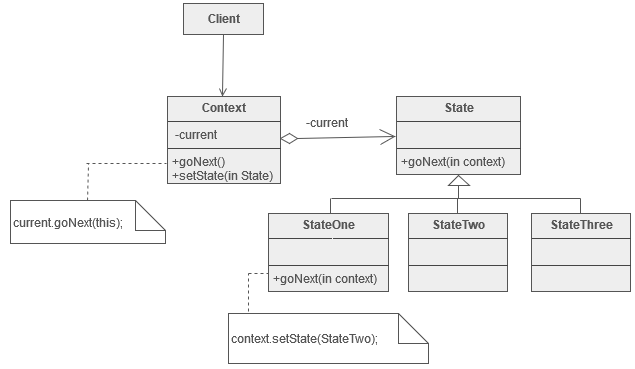
\includegraphics[width=130mm, keepaspectratio]{figures/state_static_diagram.png}
\caption{A State tervez�si minta UML oszt�lydiagrammja}
\label{fig:StatePatternClassDiagram}
\end{figure}

%----------------------------------------------------------------------------
\subsection{Generikus implement�ci�}
%----------------------------------------------------------------------------
Az el�z� megold�s alternat�v�jak�nt egy olyan megk�zel�t�s is beker�lt a motorba, mely k�zelebb �ll
a kor�bban eml�tett v�ges automat�k m�k�d�s�hez. Ez az implement�ci� mind�ssze egyetlen generikus
oszt�lyt tartalmaz, melynek neve FiniteStateMachine, ezzel is utalva a m�r eml�tett v�ges matematikai
fogalomra.

Az oszt�ly sablon param�terben kapja meg a kezelend� �llapotok t�pus�t illetve az automata bemeneteinek
t�pus�t. Emellett defini�lja azokat a t�pusokat, melyekkel meg lehet adni, hogy egy adott konkr�t automata
az �llapotokban val� tart�zkod�st illetve az �llapot�tmeneteket hogyan kezelje. Az oszt�ly m�k�d�s�nek
egyik sarkallatos pontja a bemenetek kezel�se. Ennek l�nyege, hogy az aktu�lis �llapothoz megkeresi
a bel�le kiindul� �tmeneteket, s ezek k�z�tt megkeresi, hogy melyik aktiv�l�dik az olvasott bemenet
hat�s�ra. A megold�snak Update f�ggv�nye is van, mely minden frame-ben megh�v�dik, s a kurrens �llapot
�llapotf�ggv�nyeit h�vja meg.

%----------------------------------------------------------------------------
\section{Anim�ci�s rendszer}
%----------------------------------------------------------------------------
A mai j�t�kokban gyakorlatilag b�rmilyen j�t�kobjektum rendelkezik legal�bb egy minim�lis szint�
anim�ci�val. Ezen anim�ci�k els�dleges feladata az objektumok mozg�sainak min�l �leth�bb bemutat�sa.
Emellett az anim�ci�knak inform�ci�k�zl� feladatai is lehetnek, hiszen egy gondosan fel�p�tett karakter
anim�ci�i kifejez�bbek -- �s emellett egy�rtelm�bbek, illetve k�nnyebbek �rtelmezhet�ek -- lehetnek,
mint a hangok, feliratok �s egy�b inform�ci�k�zl� form�k.

Az anim�ci�k min�s�ge teh�t nagyban meghat�rozza a j�t�kr�l alkotott v�lem�nyeket, �gy a j�t�k min�s�t�s�re,
sikeress�g�re is van befoly�suk. Nem v�letlen, hogy a nagy j�t�kfejleszt� c�gek rengeteg p�nzt �s
energi�t ford�tanak a min�l �leth�bb �s r�szletgazdagabb anim�ci�k el��ll�t�s�ra (pl.: motion capture).

Az �n rendszeremben is implement�ltam anim�ci�kkal �sszef�gg� funkci�kat, melyek a State tervez�si mint�ra
illetve az �llapotg�pes megk�zel�t�sre �p�tenek. A tov�bbiakban ezen megold�sok bemutat�sa k�vetkezik.

%----------------------------------------------------------------------------
\subsection{Csontv�z alap� anim�ci� megval�s�t�sa a State tervez�si minta felhaszn�l�s�val}
%----------------------------------------------------------------------------
Ez az implement�ci� anal�gia a State tervez�si mint�n�l le�rtakra. A tov�bbiakban az ott ismertetett
objektumoknak megfeleltethet� j�t�kmotor oldali megold�sok bemutat�sa k�vetkezik.

A State tervez�si minta State oszt�ly�nak a j�t�kmotor IState oszt�lya felel meg. Ahogy ennek az oszt�lynak a neve is sugallja, egy interf�szr�l van sz�, melynek h�rom f� absztrakt f�ggv�nye van:
az Enter f�ggv�ny az �llapotba l�p�s legelej�n, egyszer fut le, az Execute f�ggv�ny minden frame-ben
lefut, s az Exit pedig szint�n egyszer fut le, m�gpedig az �llapotb�l val� kil�p�skor. Konkr�t �llapotok
l�trehoz�s�hoz ebb�l az oszt�lyb�l kell lesz�rmazott oszt�lyokat k�sz�tenie a felhaszn�l�nak, s a megfelel�
funkci�kat az im�nt ismertetett f�ggv�nyek fel�ldefini�l�s�val adhatja meg.

A State minta ismertet�s�n�l bemutatott Context oszt�lynak a j�t�kmotor Stateable oszt�lya felel meg.
Ez az oszt�ly tagv�ltoz�k�nt elt�rolja a kurrens �llapot�t, melyet lecser�lhet, illetve befriss�t�
f�ggv�ny�ben megh�vhatja annak Execute f�ggv�ny�t.

J�t�kmotor oldalon m�g egyetlen oszt�ly, az AnimState k�pviseli ezt a megold�st, amely az IState oszt�ly
lesz�rmazottja. Ez az oszt�ly tetsz�leges sz�m� Ogre::AnimationState-et k�pes elt�rolni mag�ban (csak a
sz�m�t�g�p t�rkapacit�sa szabhat hat�rt). A szok�sos getter-setter f�ggv�nyek mellett az oszt�ly
rendelkezik egy Blend f�ggv�nnyel, mely az anim�ci�k k�z�tti �tmenetet val�s�tja meg line�ris
interpol�ci� seg�ts�g�vel.

A megold�s haszn�lat�hoz j�t�klogika-oldalon defini�lni kell egy Stateable lesz�rmazottat illetve
tetsz�leges sz�m� AnimState lesz�rmazottat (melyek lehet�s�g szerint singleton objektumok), mely
lesz�rmazottak egym�s k�z�tt d�ntik el, hogy a hozz�juk tartoz� Stateable lesz�rmazottnak mikor melyik�k
legyen az aktu�lis �llapota.

%----------------------------------------------------------------------------
\subsection{Csontv�z alap� anim�ci� megval�s�t�sa �llapotg�ppel}
%----------------------------------------------------------------------------
Ahhoz, hogy a felhaszn�l�nak ne kelljen k�zvetlen�l az Ogre anim�ci�s rendszer�t haszn�lnia,
l�trehoztam egy olyan komponenst motor oldalon, melynek az a feladata, hogy gyakran haszn�lt,
anim�ci�khoz k�t�d� m�veleteket ny�jtson a felhaszn�l�k fel�. Term�szetesen ezen m�veletek
implement�ci�i tov�bbh�vnak az Ogre anim�ci�s rendszer�be, viszont ennek k�sz�nhet�en a programoz�knak
m�r ezt nem kell megtenni�k, nekik el�g ezt az absztrah�lt interf�szt haszn�lniuk.

A kor�bban taglalt �llapotg�p implement�ci�mhoz ez �gy kapcsol�dik, hogy a felhaszn�l� j�t�k oldalon
defini�l egy AnimationComponent lesz�rmazottat, s ennek a lesz�rmazottnak a tagv�ltoz�jak�nt veheti fel
azt az egy vagy t�bb �llapotg�pet, melyek a konkr�t anim�ci�s �llapotokat �s �tmeneteiket reprezent�lj�k.

%----------------------------------------------------------------------------
\subsection{Anim�ci�s megold�sok �sszehasonl�t�sa}
%----------------------------------------------------------------------------
A State tervez�si mint�n alapul� megold�snak egy�rtelm� el�nye az �llapotg�pes megold�shoz k�pest az
anim�ci�s �llapotok interpol�l�sa �llapotv�lt�s eset�n. Ennek k�sz�nhet�en az �gy anim�lt karakterek
mozg�sa folytonosabbnak, ez�ltal �letszer�bbnek hat a felhaszn�l�k sz�m�ra.

Ennek ellen�re term�szetesen az �llapotg�pes megold�snak is megvan a maga el�nye a m�sik megold�ssal
szemben, m�gpedig az, hogy az �llapotokat le�r� f�ggv�nyek �s az �llapot�tmeneteket defini�l� f�ggv�nyek
k�djai j�l elk�l�n�lnek k�d szinten, ennek k�sz�nhet�en bonyolultabb �llapotgr�f
reprezent�l�s�ra ez a megold�s alkalmasabb, mint a State mint�n alapul� implement�ci�.

Mivel egyik megold�st sem tudtam egy�rtelm�en a jobbnak nevezni a m�sikn�l, �gy mindk�t implement�ci�
a motor r�sz�t k�pezi, s a felhaszn�l� d�nthet arr�l, hogy melyik megold�st v�lasztja a saj�t feladatai
elv�gz�s�hez.

%----------------------------------------------------------------------------
\section{Felhaszn�l�i fel�let}
%----------------------------------------------------------------------------
A felhaszn�l�i fel�letek haszn�lata a mai j�t�kokban alap funkcionalit�snak tekinthet�, hiszen m�g
egy kisebb mobil alkalmaz�snak is ny�jtania kell valamif�le GUI-t a felhaszn�l� fel�, hogy t�j�koztassa
�t a legfontosabb adatokr�l (pl.: j�t�kos �letereje), lehet�s�get adjon neki a j�t�kmenetbe t�rt�n�
beavatkoz�sra (pl.: fegyver felv�tele), vagy �ppen megv�ltoztassa az alkalmaz�s haszn�lat�nak m�dj�t
(pl.: gombok jelent�se, hanger� szab�lyoz�sa).

Ezen felsorolt jellemz�i miatt az �n rendszeremben is megval�s�tottam egy GUI rendszert a MyGUI
felhaszn�l�s�val, melyet a tov�bbiakban ismertetek.

%----------------------------------------------------------------------------
\subsection{MyGUI ismertet�se}
%----------------------------------------------------------------------------
A MyGUI egy ny�lt forr�s�, ingyenes, multiplatform GUI keretrendszer, mely MIT licensz alatt fut.
Gyorsas�ga �s egyszer�s�ge ellen�re igen komplex felhaszn�l�i fel�letek kialak�t�s�ra is alkalmas.
H�tr�nyak�nt felr�hat�, hogy a dolgozat �r�s�nak idej�n a legfrissebb stabil verzi�ja (3.2.2) 2015 janu�r
26.-�n jelent meg, teh�t az eszk�zt fejleszt� k�z�ss�g nem mutat t�lzott aktivit�st.
Ennek ellen�re sz�mos OGRE-s projektben ker�lt m�r felhaszn�l�sra, ez�rt esett r� a v�laszt�som.

Az eszk�z haszn�lat�nak kier�szakol�sa viszont nem volt z�kken�mentes. A szok�sos CMake-es kit�r�k
mellett valami�rt a program DirectX haszn�lata mellett nem volt hajland� m�k�dni. Ennek az volt az
oka, hogy az �ltalam haszn�lt OGRE verzi� (1.9) m�r a DirectX11-et haszn�lja, amelyben viszont m�r
nincs fixed function pipeline, vagyis a keretrendszer m�r nem k�n�l alap�rtelmezett �rnyal�programokat
a felhaszn�l�k sz�m�ra. Hosszas debuggol�si folyamat v�g�n der�lt csak ki, hogy ez�rt a hib��rt
a MyGUI is felel�s, hiszen neki is vannak saj�t material-jai, melye(ke)t saj�t mag�nak, bel�l �ll�t
�ssze, t�maszkodva a rendszer alap �rnyal�programjaira. A hiba jav�t�sa helyett �tt�rtem a GLSL
haszn�lat�ra, mellyel egy �jabb l�p�st tettem a multiplatforms�g fel�.

A probl�ma megold�sa ut�n a motor oldali GUI rendszert a GUI szkriptek haszn�lat�nak ir�ny�ba
fejlesztettem.

<K�PERNY�K�PEK!!!>

%----------------------------------------------------------------------------
 \section{Hangrendszer}
%----------------------------------------------------------------------------
A hangok haszn�lata a mai j�t�kokban messze t�lmutat a felhaszn�l� sz�rakoztat�s�n, hiszen emellett egy�b
c�ljai is vannak, mint p�ld�ul az aktu�lis j�t�kbeli szitu�ci�hoz kapcsol�d�
hangulat sugall�sa illetve feler�s�t�se, f�ldrajzi elhelyezked�s ismertet�se, a j�t�kost megszem�lyes�t�
karakter (vagyis az avatar) jellemz�se, vagy �ppen a j�t�kos aktu�lis cselekv�s�nek sikeress�g�t is
szok�s hangokkal jelezni a felhaszn�l� fel� (pl.: fegyver felv�tele, szintl�p�s, stb.).

�sszess�g�ben az elmondhat�, hogy a megfelel�en megv�lasztott �s id�z�tett hangokkal hatni lehet a
felhaszn�l�k lelki vil�g�ra illetve hangulat�ra, emellett inform�lj�k �ket a st�tuszukr�l, az aktu�lis k�rnyezetr�l illetve az el�rehalad�sukr�l is, s ezen tulajdons�gaik miatt a mai j�t�kok elengedhetetlen kell�kei.

Az el�bb felsorolt jellemz�k miatt az �n megold�somb�l sem hi�nyozhat egy saj�t hangrendszer implement�l�sa,
melyet az al�bbiakban ismertetek.

%----------------------------------------------------------------------------
\subsection{Megval�s�t�s}
%----------------------------------------------------------------------------
A megval�s�t�shoz az ingyenes, platformf�ggetlen OpenAL-t haszn�ltam fel, mely az OpenGL 
hang-anal�gi�j�nak is tekinthet�, legal�bbis ami az API fel�p�t�s�t tekinti. �llapotg�p!!!

Az implement�ci� ismertet�s�hez sz�ks�g van n�h�ny OpenAL-hez kapcsol�d� fogalom tiszt�z�s�ra, melyeket
a k�vetkez�kben ismertetek.

A listener az a t�rbeli objektum, melynek a szemsz�g�b�l renderelj�k a hangforr�sokat (pongyol�n
fogalmazva ez a kamera f�le). A defin�ci�j�b�l ad�dik, hogy egyid�ben csak egyetlen ilyen
objektumnak kell l�teznie, jelenett�l f�ggetlen�l.

A buffer objektum megfeleltethet� egy olyan le�r� f�jlnak, mely egy hangf�jl adatait 
tartalmazza. Ilyen t�pus� objektumb�l ak�rh�nyat fel lehet haszn�lni.

A source olyan objektum, mely egy vagy t�bb buffer lej�tsz�s�t teszi lehet�v�. T�bb source-hoz is
hozz� lehet rendelni ugyan azt a buffert, viszont egy source egyszerre csak egyetlen buffer tartalm�t
k�pes emitt�lni. Ebb�l m�r nem lehet
egyszerre ak�rmennyi a rendszerben, hiszen a hangk�rty�k hardveres limit�ci�i ezt nem teszik lehet�v�.
Az �n megold�somban maximum 16 buffer tartalm�t lehet lej�tszani egyid�ben, �gy a megold�som r�gebbi
hangk�rty�kkal is kompatibilis.
A forr�s objektumokkal kapcsolatban megjegyzend�, hogy lehetnek 2D-sek (Music vagy Ambient)
illetve 3D-sek (SoundEffect) is. Az el�bbi
azt jelenti, hogy a listenert�l val� t�vols�ga mindig nulla, m�g �rtelemszer�en ez a 3D-s esetben nem
igaz. A h�romdimenzi�s (azaz t�rbeli) hangokn�l a val�s�gh�bb hang�rzet el�r�s�nek �rdek�ben a
hangmagass�got megperturb�lom egy �ltalam megv�lasztott random faktorral. A tov�bbi val�s�gh� �rzet
kelt�se �rdek�ben nem csak a hangmagass�got, hanem a kiv�laszott buffert is randomiz�lhatja a felhaszn�l�,
ha akarja (de d�nthet �gy is, hogy a source-hoz rendelt buffereket sorrendhelyesen akarja lej�tszani).
Ennek implement�l�s�hoz ki kellett vennem a rendszerb�l az OpenAL be�p�tett looping funkcionalit�s�t,
ugyanis az a bufferek cser�lget�s�t nem hordozza mag�ban.

A megval�s�t�shoz k�t oszt�lyt defini�ltam motor oldalon. Az egyik az AudioManager, melynek feladata
a source-ok, a bufferek �s a listener menedzsel�se �s karbantart�sa. A m�sik objektum az
AudioSourceComponent, mely szabad source-ot �s tetsz�leges sz�m� buffert k�rhet az AudioManager-t�l,
s lej�tszhatja a hozz� rendelt buffereket tetsz�leges sz�m� alkalommal, a kor�bban eml�tett m�dokon.
Ha az AudioManager nem tud adni az AudioSourceComponent-nek szabad source-ot, akkor a lej�tsz�s
egyszer�en nem t�rt�nik meg, de a rendszerben att�l m�g megjelenik az ig�ny.
Az AudioManager teh�t tetsz�leges sz�m� AudioSourceComponent-et menedzsel, s minden frame-ben
fel�ll�t k�zt�k egy sorrendis�get a k�vetkez�k szerint: legel�re veszi a Music t�pus� komponenseket,
azt�n az Ambient t�pus�ak k�vetkeznek, v�g�l pedig a SoundEffect-ek maradnak, melyek k�z�tti sorrendet
a listenert�l val� t�vols�g hat�rozza meg (a k�zelebbi ker�l el�r�bb a sorban).
Az �gy berendezett t�rol� els� 16 eleme OpenAL source-hoz jut, a t�bbi pedig v�rakozni k�nyszer�l.

<DIAGRAMOK!!!>

%----------------------------------------------------------------------------
\section{Plak�tok �s r�szecskerendszerek}
%----------------------------------------------------------------------------
Nem volt ig�ny k�d oldali reprezent�ci�ra, mind�ssze annyib�l �ll az implement�ci�, hogy egy
speci�lis motor oldali komponens (ParticleComponent) k�pes beparszolni illetve le�ll�tani/�jraind�tani
egy Ogre ParticleScriptet. Ez a megold�s az�rt el�ny�s, mert a r�szecskerendszer m�dosul�sa eset�n
nem kell �jraford�tani a forr�sk�dot. Emellett viszont ez a megk�zel�t�s nem teszi lehet�v�
r�szecskerendszerek k�db�l t�rt�n� m�dos�t�s�t vagy ak�r l�trehoz�s�t.

talan lehetne felhozni itt egy pl scriptet?
%----------------------------------------------------------------------------
\section{Egy�b}
%----------------------------------------------------------------------------
Delegate

%----------------------------------------------------------------------------
\section{�ttekint�s}
%----------------------------------------------------------------------------

<DIAGRAMOK!!!>

%----------------------------------------------------------------------------
\chapter{Demonstr�ci�s alkalmaz�s}\label{sect:DemoApp}
%----------------------------------------------------------------------------
Ez a fejezet a j�t�kmotor m�k�d�s�nek demonstr�l�s�ra k�sz�tett p�lda alkalmaz�st mutatja be.
El�sz�r is tiszt�zza az alkalmaz�ssal szemben t�masztott k�vetelm�nyeket, azt�n kit�r a megval�s�t�s
r�szleteire is, majd az elk�sz�lt alkalmaz�s �ttekint�se ut�n a tesztel�si eredm�nyek taglal�s�val
z�rul.

%----------------------------------------------------------------------------
\section{K�vetelm�nyek}
%----------------------------------------------------------------------------
A k�vetelm�nyek meghat�roz�sakor arra kellett t�rekednem, hogy az elk�sz�tett motor k�pess�geire
min�l jobban t�maszkodjon az elk�sz�tend� demonstr�ci�s alkalmaz�s. Fontos szempont volt tov�bb� az is, hogy
a p�lda alkalmaz�snak "legyen �rtelme", vagyis legyen kezdeti �llapota �s c�lja, illetve hogy
ne csak nyerni, hanem veszteni is lehessen benne.

Ezen szempontokat is figyelembe v�ve egy z�rt t�rben j�tsz�d� FPS (First Person Shooter) j�t�k
megval�s�t�s�ra v�llalkoztam, ahol a felhaszn�l� �ltal ir�ny�tott j�t�kosnak nincsenek seg�t�i, csak
ellenfelei, melyek a p�lya adott pontjain jelenhetnek meg, s moh� m�don a j�t�kos fel� tartanak, ha
�leterej�k nagyobb, mint egy, k�l�nben menek�lnek a j�t�kos el�l. Az ellens�ges objektumok hull�mokban
jelennek meg a sz�nt�ren, m�gpedig �gy, hogy az n. hull�m kezdetekor 2n darab �j ellens�ges objektum
keletkezik. Az ellens�ges objektumok sz�m�ra nincs fels� korl�t, ilyen �rtelemben ez egy v�gtelen�tett
j�t�k, amelynek csak akkor van v�ge, ha a j�t�kos karakter�nek az �letereje null�ra cs�kken.

%----------------------------------------------------------------------------
\section{Megval�s�t�s}
%----------------------------------------------------------------------------
Ez a szakasz az alkalmaz�s sor�n megval�s�tott fontosabb oszt�lyok bemutat�s�t tartalmazza.

%----------------------------------------------------------------------------
\subsection{DynamicMovementComponent}
%----------------------------------------------------------------------------
Ennek a komponens lesz�rmazottnak az a feladata, hogy dinamikus fizikai komponenssel rendelkez�
j�t�kobjektum felhaszn�l�i inputokkal t�rt�n� transzform�l�s�t megoldja illetve a fizikai �tk�z�sekkor
bek�vetkez� esem�nyeket lekezel� f�ggv�nyek defini�l�s�t megtegye. Ennek megfelel�en ez a komponens
felel a felhaszn�l�t reprezent�l� karakter transzform�ci�j�nak m�dos�t�s��rt (\figref{DemoAppUnarmedRun} �bra).

\begin{figure}[!ht]
\centering
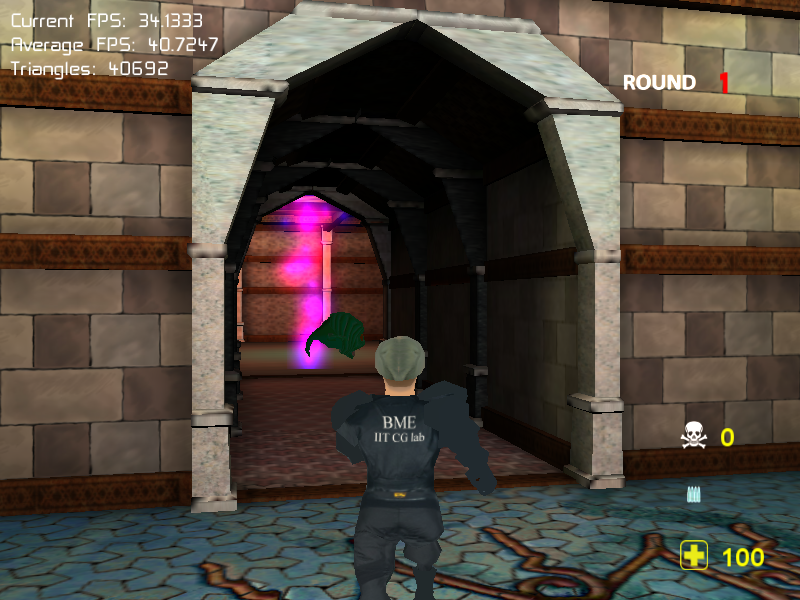
\includegraphics[width=100mm, keepaspectratio]{figures/demoapp_unarmed_run.png}
\caption{P�lda a j�t�kos karakter�nek transzform�l�s�ra.}
\label{fig:DemoAppUnarmedRun}
\end{figure}

%----------------------------------------------------------------------------
\subsection{EnemyAIComponent}
%----------------------------------------------------------------------------
Ez a komponens lesz�rmazott nagyon hasonl�t az el�z�ekben ismertetett \verb+DynamicMovementComponent+
oszt�lyhoz, ugyanis ez az oszt�ly is dinamikus fizikai komponenssel rendelkez� objektum transzform�l�s�t
�s az �tk�z�seinek kezel�s�t v�gzi, annyi k�l�nbs�ggel, hogy ebben az esetben nem a felhaszn�l�i
bemenetek, hanem egy bels� logika d�nt az elmozdul�s �s az elforgat�s milyens�g�r�l. Ahogy arra a
komponens nev�b�l is k�vetkeztetni lehet, ez az oszt�ly felel�s az ellens�ges j�t�kobektumok
transzform�ci�j�nak m�dos�t�s��rt.

A megval�s�t�s sor�n 4 �llapotot defini�ltam az ellens�ges karakterek sz�m�ra, ezek rendre a \verb+Search+,
\verb+Attack+, \verb+RunAway+ �s \verb+Dead+ �llapotok (\figref{EnemyAIStateGraph} �bra). Az �llapotokhoz tartoz�
f�ggv�nyeket illetve az �llapot�tmenetek
menedzsel�s�t a motor oldali generikus �llapotg�p seg�ts�g�vel, a \verb+FiniteStateMachine+ oszt�ly
felhaszn�l�s�val val�s�tottam meg. Ami az implement�ci� mesters�ges intelligenci�ra vonatkoz� r�sz�t
illeti, az �llapotg�phez rendelt �llapotf�ggv�nyeknek az a feladatuk, hogy a felhaszn�l� �ltal
ir�ny�tott karakterhez k�pest meghat�rozza az k�v�nt elmozdul�s ir�ny�t �s az elforgat�s sz�g�t, s ezeknek
megfelel�en er�k illetve forgat�nyomat�kok seg�ts�g�vel elv�gzi a sz�ks�ges transzform�ci�kat.
L�that�, hogy ez a megold�s meglehet�sen korl�tozott intelligenci�t ruh�z az ellens�ges j�t�kobjektumokra,
hiszen mivel ez egy moh� algoritmus (azaz mindig az aktu�lis �llapot alapj�n d�nt, determinisztikusan),
�gy p�ld�ul az akad�lyok kiker�l�se, a kooper�ci� stb. nem megoldhat� ezzel a megval�s�t�ssal.

\begin{figure}[!ht]
\centering
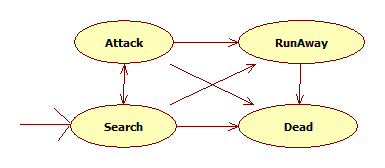
\includegraphics[width=70mm, keepaspectratio]{figures/enemyAIState.png}
\caption{Az ellens�ges objektumok mesters�ges intelligenci�j�nak �llapotgr�fja.}
\label{fig:EnemyAIStateGraph}
\end{figure}

%----------------------------------------------------------------------------
\subsection{EnemyAnimationComponent}
%----------------------------------------------------------------------------
Ennek az \verb+AnimationComponent+-lesz�rmazottnak az a feladata, hogy az ellens�ges j�t�kobjektumok anim�l�s�t
menedzselje a motor oldali \verb+FiniteStateMachine+ oszt�ly seg�ts�g�vel.

Az implement�ci� sor�n 3 anim�ci�s �llapotot defini�ltam, ezek rendre a \verb+Walk+, \verb+Attack+ �s \verb+Dead+
�llapotok (\figref{EnemyAnimStateGraph} �bra). Term�szetesen ezek az �llapotok �sszef�ggnek az im�nt ismertetett \verb+EnemyAIComponent+-ben
defini�lt �llapotokkal a k�vetkez� m�don: amikor az \verb+EnemyAIComponent+ \verb+Search+ vagy \verb+RunAway+
�llapotban van, akkor az \verb+EnemyAnimationComponent+ \verb+Walk+ �llapotban, illetve minden m�s
\verb+EnemyAIComponent+-beli �llapothoz a vele megegyez� nev� \verb+EnemyAnimationComponent+-beli �llapot tartozik.

\begin{figure}[!ht]
\centering
\includegraphics[width=70mm, keepaspectratio]{figures/EnemyAnimState.png}
\caption{Az ellens�ges objektumok anim�ci�j�nak �llapotgr�fja.}
\label{fig:EnemyAnimStateGraph}
\end{figure}

%----------------------------------------------------------------------------
\subsection{GUIComponent}
%----------------------------------------------------------------------------
Ez a komponens-lesz�rmazott felel a MyGUI szkriptek seg�ts�g�vel defini�lt felhaszn�l�i fel�let
menedzsel�s��rt, amibe beletartozik a men�elemekhez k�t�d� esem�nyek kezel�se illetve mag�nak a men�nek
a megjelen�t�se �s elrejt�se a j�t�kmenet aktu�lis �llapot�nak megfelel�en. A p�lda alkalmaz�somban
ez az egyetlen olyan komponens, mely dinamikus (azaz reszponz�v) felhaszn�l�i fel�letet val�s�t meg.

A p�lda alkalmaz�sban felhaszn�lt, MyGUI seg�ts�g�vel megalkotott felhaszn�l�i fel�let a \figref{MyGUI_Example}
�br�n l�that�.

\begin{figure}[!ht]
\centering
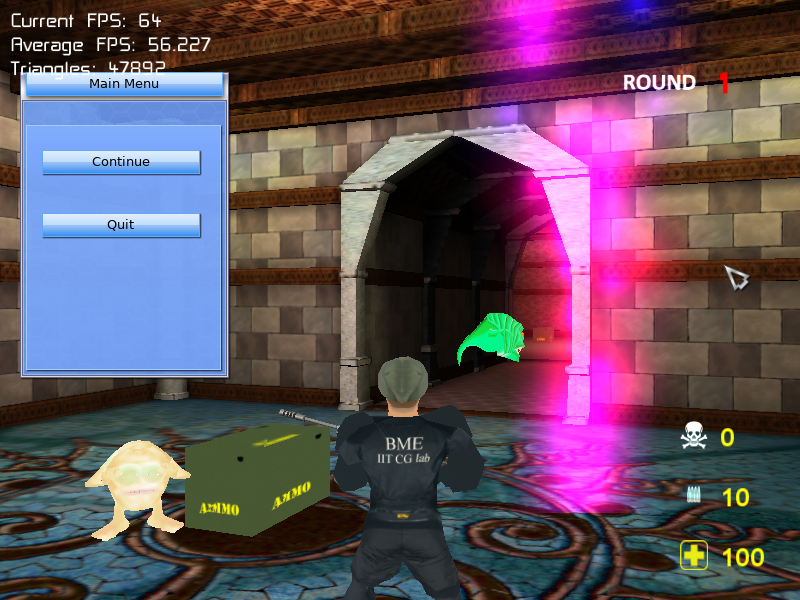
\includegraphics[width=100mm, keepaspectratio]{figures/mygui_example.png}
\caption{Reszponz�v felhaszn�l�i fel�let kialak�t�sa a MyGUI felhaszn�l�s�val.}
\label{fig:MyGUI_Example}
\end{figure}

%----------------------------------------------------------------------------
\subsection{HUDComponent}
%----------------------------------------------------------------------------
Ez a komponens lesz�rmazott is -- a kor�bbiakban ismertetett \verb+GUIComponent+-hez hasonl�an -- felhaszn�l�i
fel�let menedzsel�s�vel foglalkozik, annyi k�l�nbs�ggel, hogy ez az oszt�ly az Ogre Overlay keretrendszert
haszn�lja a felhaszn�l� sz�m�ra fontosnak tartott inform�ci�k
(aktu�lis �letpont, aktu�lis t�lt�nyek sz�ma, meg�lt ellenfelek sz�ma illetve az aktu�lis k�r sorsz�ma) k�perny�n
t�rt�n� megjelen�t�s�re. Ennek megfelel�en az ezzel a komponenssel megjelen�tett felhaszn�l�i fel�let --
a GUIComponent-�vel ellent�tben -- statikus, nem pedig dinamikus, vagyis felhaszn�l�i esem�nyekre nem k�pes
reag�lni.

A demonstr�ci�s alkalmaz�sban informat�v szerepet bet�lt� statikus felhaszn�l�i fel�letre mutat p�ld�t a
\figref{DemoAppKill} �bra.

\begin{figure}[!ht]
\centering
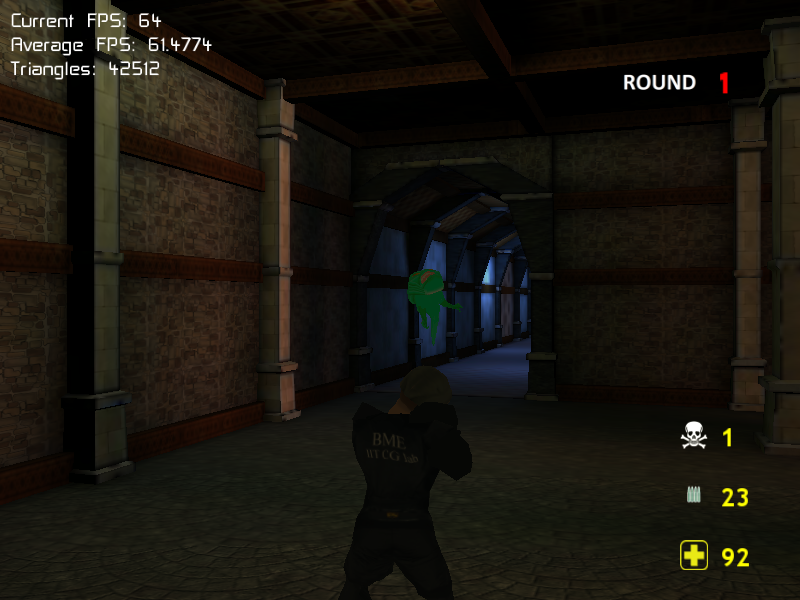
\includegraphics[width=100mm, keepaspectratio]{figures/demoapp_kill.png}
\caption{P�lda a statikus felhaszn�l�i fel�let informat�v szerep�re.}
\label{fig:DemoAppKill}
\end{figure}

%----------------------------------------------------------------------------
\subsection{ManagerComponent}
%----------------------------------------------------------------------------
Ez a komponens-lesz�rmazott felel a p�ly�n megjelen� ellens�ges j�t�kobjektumok megfelel� �temben
�s helyen t�rt�n� l�trehoz�s��rt. Emellett ennek az oszt�lynak a feladata az is, hogy a \verb+HUDComponent+-et
t�j�koztassa a sz�ks�ges mennyis�gek aktu�lis �rt�keir�l. Ennek megval�s�t�s�hoz felhaszn�lja a j�t�kost reprezent�l�
objektumhoz rendelt \verb+PlayerDataComponent+-et (\sectref{PlayerDataComponent}. alszakasz) �s
\verb+WeaponComponent+-et (\sectref{WeaponComponent}. alszakasz) egyar�nt.

%----------------------------------------------------------------------------
\subsection{PlayerDataComponent}\label{sect:PlayerDataComponent}
%----------------------------------------------------------------------------
Ennek a komponensnek az a feladata, hogy a felhaszn�l� �ltal ir�ny�tott karakter illetve az ellens�ges
j�t�kobjektumok legfontosabb k�z�s tulajdons�gait (�leter�, meg�lt ellenfelek sz�ma illetve egy flag
arr�l, hogy van-e n�la fegyver) menedzselje.

%----------------------------------------------------------------------------
\subsection{SoldierAnimationComponent}
%----------------------------------------------------------------------------
Ez a speci�lis \verb+AnimationComponent+ az�rt felel, hogy a felhaszn�l� �ltal ir�ny�tott j�t�kobjektum
mindig a megfelel� anim�ci�val legyen ell�tva.

Implement�ci�s szinten ez az oszt�ly �gy viszonyul a \verb+DynamicMovementComponent+-hez, mint ahogy
az \verb+EnemyAnimationComponent+ viszonyult az \verb+EnemyAIComponent+-hez, annyi k�l�nbs�ggel, hogy a
\verb+DynamicMovementComponent+-ben nincs �llapothalmaz, viszont ebben az oszt�lyban kett� is van.

A k�t �llapothalmazra az�rt van sz�ks�g, mert a felhaszn�l� �ltal ir�ny�tott j�t�kobjektum
anim�ci�inak nagy r�sze vagy csak a karakter fels� test�re, vagy csak annak az als� test�re vonatkozik,
ennek megfelel�en a k�l�nb�z� halmazokban lev� �llapotok egym�st�l f�ggetlen�l kezelend�k. Ez k�dszinten
azt jelenti, hogy k�t \verb+FiniteStateMachine+ p�ld�nyt kell menedzselnie ennek az oszt�lynak.

Az als� testre vonatkoz� �llapothalmaz �llapotait az \verb+Idle+, \verb+Run+ �s \verb+Dead+ �llapotok alkotj�k, m�g
a fels� testen haszn�latos �llapothalmazba az \verb+Idle+, \verb+Run+, \verb+WeaponHold+, \verb+Shoot+ �s \verb+Dead+
�llapotok tartoznak (\figref{SoldierAnimStateGraph} �bra). Megjegyzend�, hogy az �llapotok �s az anim�ci�k k�z�tt nem
egy�rtelm� a lek�pez�s, hiszen a death anim�ci� (\figref{DemoAppDead} �bra) mind az als� testre, mind a fels� testre
vonatkozik, viszont mindk�t �llapotg�pben szerepel a hozz� tartoz� �llapot a helyes m�k�d�s el�id�z�se �rdek�ben.

\begin{figure}[!ht]
\centering
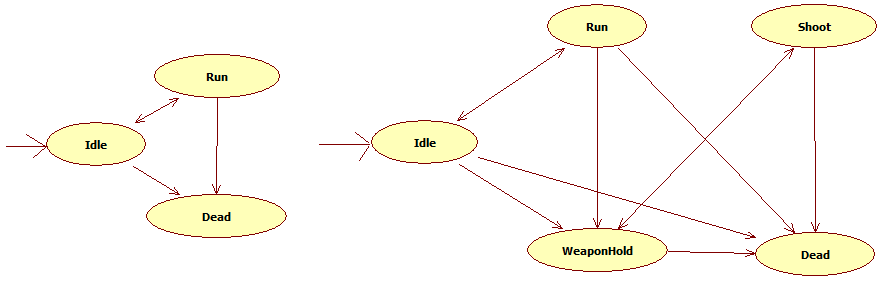
\includegraphics[width=150mm, keepaspectratio]{figures/soldierAnimState.png}
\caption{A felhaszn�l� �ltal ir�ny�tott karakter als�- illetve fels�testre vonatkoz� anim�ci�s gr�fjai.}
\label{fig:SoldierAnimStateGraph}
\end{figure}

\begin{figure}[!ht]
\centering
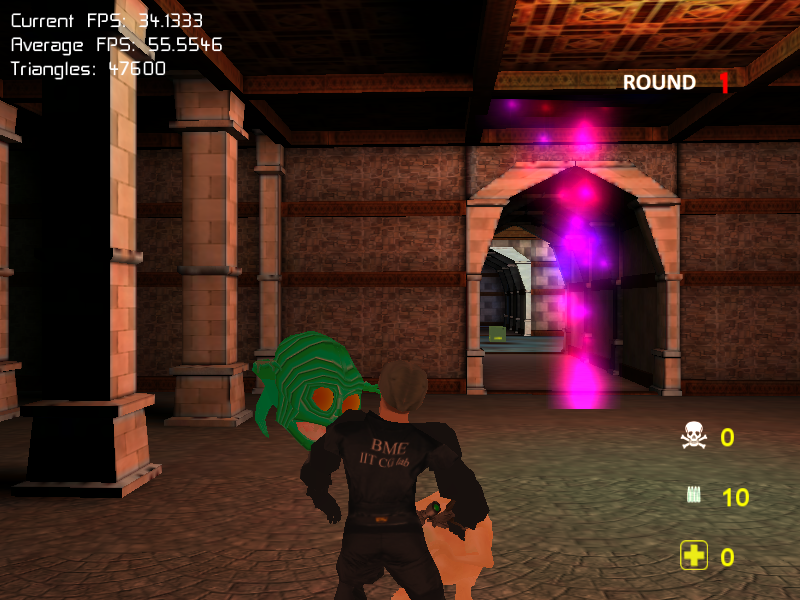
\includegraphics[width=100mm, keepaspectratio]{figures/demoapp_dead.png}
\caption{Az ellens�ges karakterek elpuszt�tj�k a felhaszn�l� �ltal ir�ny�tott j�t�kobjektumot.}
\label{fig:DemoAppDead}
\end{figure}

%----------------------------------------------------------------------------
\subsection{SoldierAnimComponent}
%----------------------------------------------------------------------------
A \sectref{Engine}. fejezetben le�rtaknak megfelel�en nem csak a \verb+FiniteStateMachine+ oszt�ly felhaszn�l�s�val,
hanem a State tervez�si minta alkalmaz�s�val is lehet �llapotg�p funkci�kat megval�s�tani.

Ez az oszt�ly a neve ellen�re nem komponens, hanem \verb+Stateable+ lesz�rmazott, ennek megfelel�en
\verb+IState+ lesz�rmazottak seg�ts�g�vel meg lehet adni a mindenkori aktu�lis �llapot�t. Az oszt�ly nev�ben az�rt szerepel
m�gis a Component ut�tag, mert ezzel is szerettem volna arra utalni, hogy haszn�lhat�s�g�t tekintve nem sokban k�l�nb�zik
b�rmely \verb+Component+ lesz�rmazott�l.
Ehhez defini�ltam h�rom darab \verb+AnimState+ lesz�rmazottat, melyek singleton objektumok, s egym�s k�z�tt
d�ntik el, hogy adott felt�telek eset�n melyik�k legyen a hozz�juk tartoz� \verb+SoldierAnimComponent+
p�ld�ny aktu�lis �llapota. Az elk�sz�tett rendszer szerepl�it illetve azok kapcsolatait a \figref{GameSideStateHierarchy}
�bra foglalja �ssze.

\begin{figure}[!ht]
\centering
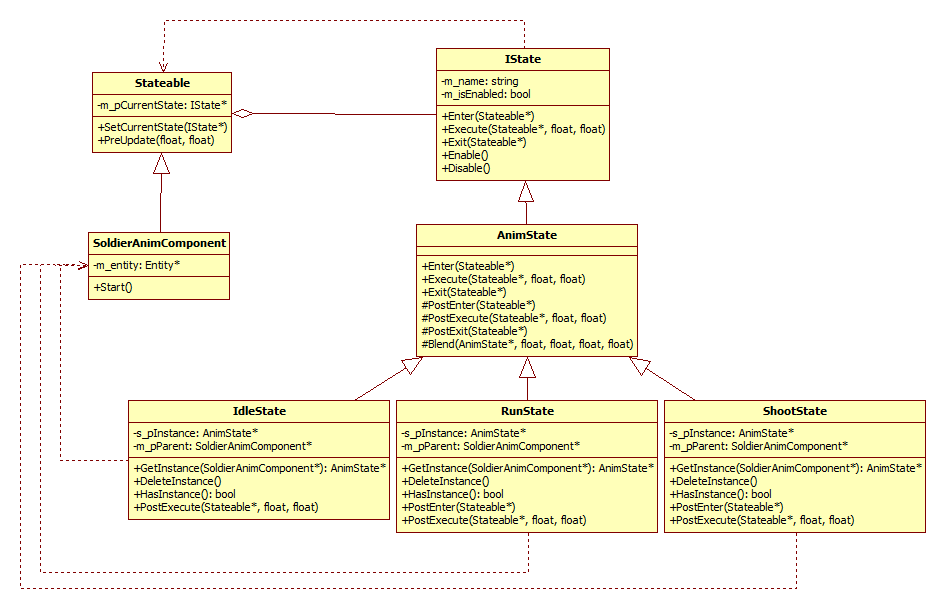
\includegraphics[width=150mm, keepaspectratio]{figures/demoapp_state.png}
\caption{A rendszeremben megval�s�tott State tervez�si minta UML oszt�lydiagrammja.}
\label{fig:GameSideStateHierarchy}
\end{figure}

%----------------------------------------------------------------------------
\subsection{WeaponComponent}\label{sect:WeaponComponent}
%----------------------------------------------------------------------------
Ez a komponens menedzseli a j�t�kos karaktere �ltal felvehet� fegyver objektumot. A menedzsel�sbe
beletartozik a t�lt�nyek sz�m�nak kezel�se, illetve maga a l�v�si folyamat defini�l�sa is, mely sor�n
a fizikai rendszer seg�ts�g�vel fizikai first hit raycasting-ot haszn�lva a fegyver cs�v�b�l l�tt
sug�rral metszi el a sz�nteret, s az els�k�nt eltal�lt fizikai objektumt�l von le �letet akkor, ha az
az objektum egy ellens�ges karakter volt (azt, hogy egy j�t�kobjektum ellens�g-e, a hozz� rendelt tag-ek
alapj�n lehet eld�nteni). Mindezek mellett szint�n ennek a komponensnek a feladata, hogy
a sz�l� j�t�kobjektumhoz k�pest megfelel� transzform�ci�val l�ssa el a fegyvert reprezent�l�
j�t�kobjektumot. Ezt �gy val�s�tja meg, hogy a sz�l� j�t�kobjektum jobb kez�hez k�pest alkalmaz
egy x tengely k�r�li, 90�-os elforgat�st (\figref{WeaponHoldDemo} �bra).

\begin{figure}[!ht]
\centering
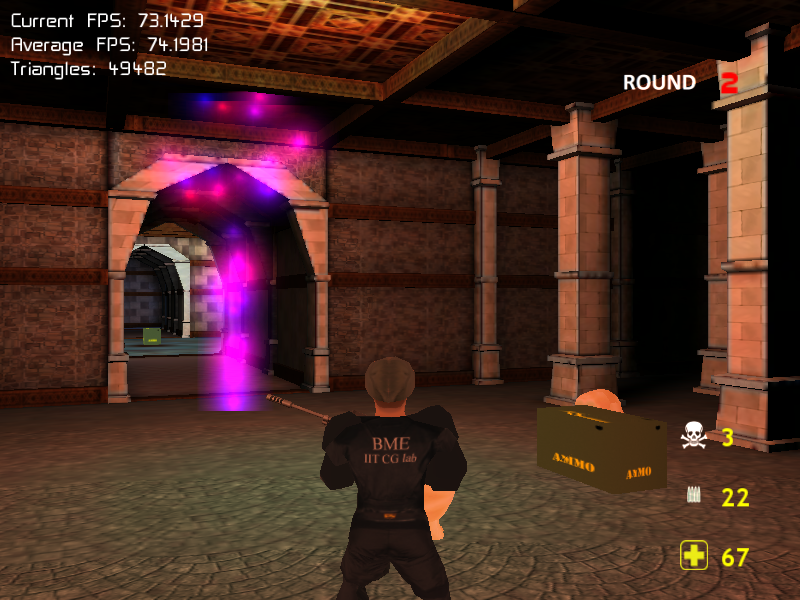
\includegraphics[width=100mm, keepaspectratio]{figures/weapon_transform.png}
\caption{A fegyver helyzete a katona kez�hez igaz�tva.}
\label{fig:WeaponHoldDemo}
\end{figure}

%----------------------------------------------------------------------------
\section{�ttekint�s}
%----------------------------------------------------------------------------
Az im�nt ismertetett j�t�klogika-oldali komponensek kapcsolatait �sszefoglal� UML oszt�lydiagramm
a \figref{GameSideCompHierarchy} �br�n l�that�.

\begin{figure}[!ht]
\centering
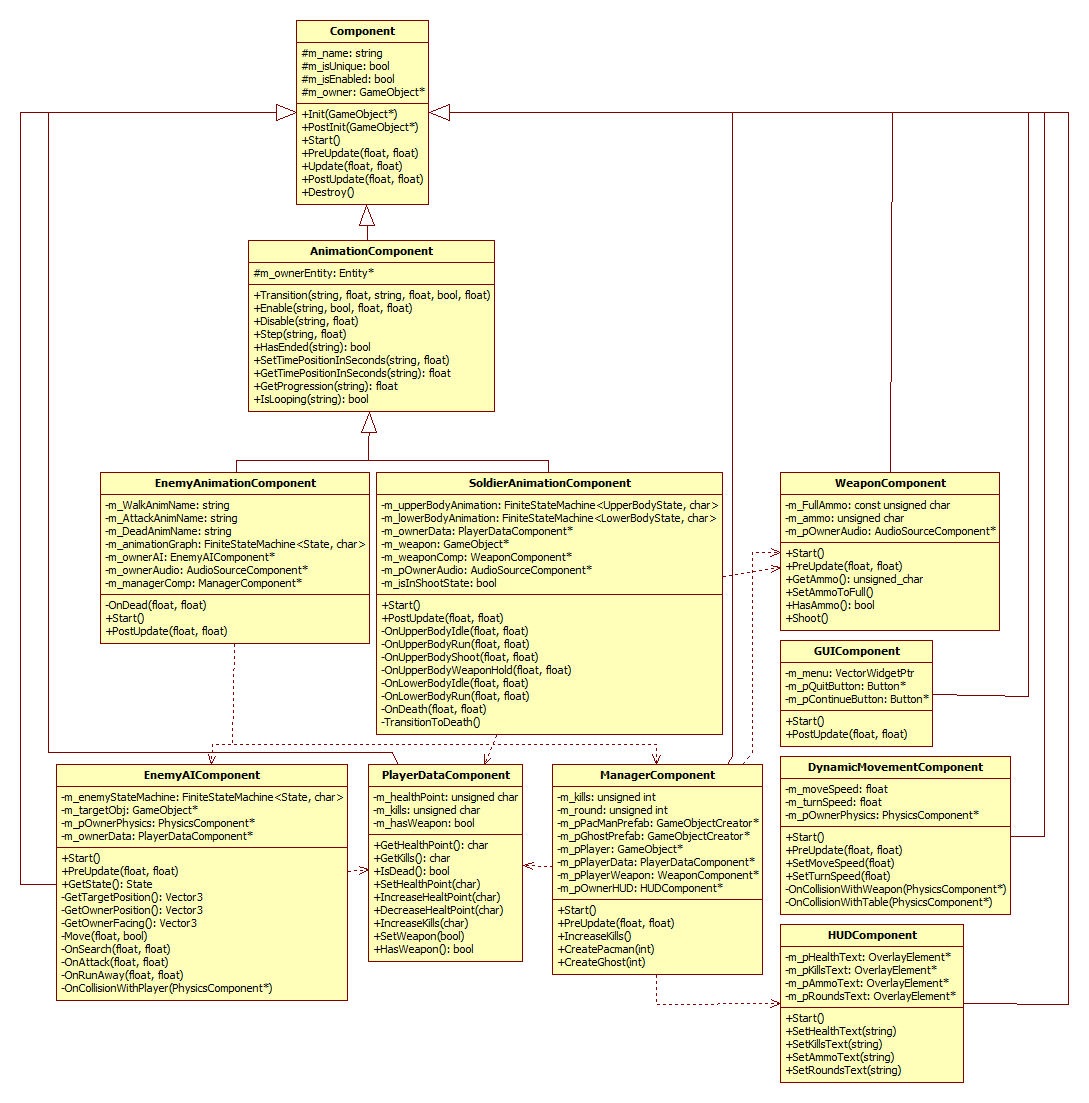
\includegraphics[width=150mm, keepaspectratio]{figures/gameside_comp_hierarchy.png}
\caption{A j�t�klogika oldalon elk�sz�tett fontosabb komponensek UML oszt�lydiagrammja.}
\label{fig:GameSideCompHierarchy}
\end{figure}

%----------------------------------------------------------------------------
\chapter{�rt�kel�s}
%----------------------------------------------------------------------------
Ez a fejezet az elk�sz�lt j�t�kmotorom �rt�kel�s�vel foglalkozik. Els�k�nt megvizsg�lja, hogy
az el�z� fejezetben ismertetett demonstr�ci�s alkalmaz�s elk�sz�t�se mennyire volt egyszer�,
majd kit�r az elk�sz�lt k�d teljes�tm�ny�re.

%----------------------------------------------------------------------------
\section{Haszn�lhat�s�g}
%----------------------------------------------------------------------------
Ez a szakasz megvizsg�lja a diplomaterv keret�ben elk�sz�tett �ltal�nos c�l�, komponens alap�
j�t�kmotort annak haszn�lhat�s�ga szempontj�b�l. Ez egy olyan metrika, melyet neh�z m�rni,
hiszen alapvet�en szubjekt�v v�lem�nyt t�kr�z. Valamif�le �rt�kel�sre m�giscsak sz�ks�g van,
hiszen az elk�sz�lt rendszerem egyik legfontosabb min�s�t�se annak haszn�lhat�s�ga.

A demonstr�ci�s alkalmaz�sn�l le�rtaknak megfelel�en j�t�klogika oldalon szinte kiz�r�lag
komponenseket k�sz�tettem (illetve egy main f�ggv�nyt, ahol a j�t�k ind�t�s�hoz sz�ks�ges teend�ket
v�geztem el �s egy XML parser oszt�lyt a DynamicMovementComponent oszt�ly sz�m�ra). Ezen j�t�klogika
oldali komponensek forr�sf�jlainak �sszm�rete
1387 sor, s 11 ilyen komponenst defini�ltam (nem mindet ismerettem az el�z� fejezetben,
csak a legfontosabbakat), vagyis komponensenk�nt k�r�lbel�l 126
sornyi k�dot kellett �rnom, ami v�lem�nyem szerint nem nevezhet� soknak. Ebb�l k�vetkezik, hogy a
j�t�klogika oldali k�dok a sok funkcionalit�s elv�gz�s�t kev�s k�ddal val�s�tj�k meg, teh�t a j�t�koldali
komponensek nagym�rt�kben t�maszkodnak az elk�sz�tett j�t�kmotorom k�pess�geire.

Az el�z� fejezetben le�rtaknak megfelel�en a demonstraci�s alkalmaz�s megalkot�sa sor�n nem kellett alacsonyszint� grafikai m�veleteket
-- mint p�ld�ul pufferek kezel�se, �rnyal�programok param�tereinek el��ll�t�sa stb. -- v�geznem, hiszen ezeket a teend�ket az elk�sz�tett
j�t�kmotorom l�tta el. S�t, enn�l magasabb szint� funkcionalit�sok megval�s�t�s�nak terh�t is levette r�lam a motor, hiszen nem kellett
f�nyforr�sokkal illetve anyagjellemz�kkel foglalkoznom (az OGRE-ben �rt anyagle�r� szkriptek �s a j�t�klogika oldalon megval�s�tott
�rnyal�programok mellett), emellett a fizik�val kapcsolatos funkcionalit�sokat is csak haszn�lnom kellett j�t�klogika oldalon, ami szint�n
nagyban megk�nny�tette a dolgomat. Mindezek mellett szint�n nem kellett foglalkoznom a felhaszn�l�i bemenetek kezel�s�vel illetve a j�t�k
f�hurk�t sem nekem kellett elk�sz�tenem, hiszen ezek a funkcionalit�sok is a m�r kor�bban elk�sz�tett j�t�kmotorom r�sz�t k�pezt�k.
A motor minden alrendszere -- megjelen�t�s, fizika, hang, stb. -- egys�ges m�don kezelhet�, a felhaszn�l�nak
nem kell ismernie a bels� m�k�d�seiket a haszn�latukhoz, viszont a rendszer lehet�s�get ad arra is -- t�bb m�s motorral ellent�tben --, hogy
a hozz��rt� felhaszn�l�k k�zvetlen�l hozz�f�rhessenek a k�l�nf�le almotorokhoz, �gy nem csak azok kivezetett funkcionalit�sait �rhetik el. 

Ami a komponens alap� megk�zel�t�st illeti, v�lem�nyem szerint k�nyelmes volt �j komponenseket adni a rendszerhez, hiszen a legt�bb esetben
csak n�h�ny f�ggv�ny fel�ldefini�l�s�ra volt sz�ks�g. A komponensek k�z�tti kommunik�ci� haszn�lata sem okozott probl�m�t, hiszen
a megfelel� kont�ner oszt�lyokt�l tort�n� lek�rdez�seken t�l nem volt m�s feladatom ezzel kapcsolatban. Hat�konys�gi okokb�l arra kellett
figyelnem, hogy a lek�rdez�seket ne minden k�pkocka kisz�m�t�s�ra v�gezzem el, hanem ahol erre lehet�s�g volt, ott a lek�rdezend� komponenst
illetve j�t�kobjektumot tagv�ltoz�k�nt elt�roltam abban az oszt�lyban, mely azt haszn�lni akarta.

Az elk�sz�tett rendszerem eddig felsorolt tagjai mellett m�g a j�t�kobjektumok k�sleltetett l�trehoz�s�ra szeretn�k kit�rni. Ez a funkcionalit�s
nagyban megk�nny�tette egy komponens illetve egy j�t�kobjektum le�r�s�nak �jrafelhaszn�l�s�t mind XML, mind C\texttt{++} oldalon.

%----------------------------------------------------------------------------
\section{Teljes�tm�ny}
%----------------------------------------------------------------------------
K�l�nb�z� �ssze�ll�t�s� sz�ntereken v�geztem m�r�seket, melyek eredm�nyeit az al�bbiakban ismertetem.
A m�r�sekkel kapcsolatosan megjegyzend�, hogy mindegyiket egy percig v�geztem, s a kurrens
illetve az �tlagos FPS (Frames per Seconds, k�pkockasebess�g) jelenik meg a k�perny�k�peken
(a h�romsz�gek sz�ma mellett).

A m�r�sekkel kapcsolatosan megjegyzend�, hogy az Ogre be�p�tett, FPS-re vonatkoz� lek�rdez� f�ggv�nyeit nem
haszn�lhattam, mivel ezek az Ogre be�p�tett megjelen�t�si hurk�t haszn�lj�k fel az implement�ci�juk sor�n,
viszont az �n rendszeremben saj�t megjelen�t�si hurkot defini�ltam. Ennek megfelel�en a motorban lev�,
megjelen�t�s�rt felel�s alrendszerben implement�lnom kellett az FPS sz�mol�shoz sz�ks�ges logik�t. Ennek megval�s�t�sa
sor�n arra t�rekedtem, hogy ez a logika min�l egyszer�bb legyen annak �rdek�ben, hogy
a m�r�s min�l kisebb sz�zal�kban befoly�solja a m�r�si eredm�nyt. �gy v�lem, hogy ezt siker�lt is el�rnem,
hiszen a kurrens illetve az �tlag k�pkockasebess�g m�r�s�hez mind�ssze egyetlen 32 bites lebeg�pontos statikus v�ltoz�t
illetve egy 32 bites sz�ml�l�t haszn�ltam fel. A gyors lek�rdez�sek �rdek�ben a k�v�nt �rt�keket tagv�ltoz�kban t�roltam el.
A megold�s fontosabb r�szleteit az al�bbi k�dr�szlet szeml�lteti.

\begin{lstlisting}[frame=single,float=!ht,
caption={Saj�t FPS-sz�mol�s implement�l�s�nak fontosabb r�szletei.}, label=ForwardDeclarationCpp]
void RenderSystem::Update (float t, float dt)
{
	static float sumFPS = 0.0f;
	static unsigned int count = 0;

	// ...

	if (/*...*/) {
		// ...
		m_currentFPS = 1 / dt;
		sumFPS += m_currentFPS;
		++count;
		m_averageFPS = sumFPS / count;
	}

	// ...
}
\end{lstlisting}

A m�r�seket a laptopomon v�geztem el, melynek fontosabb adatait a \tabref{HWConfigTable} t�bl�zat foglalja �ssze:

\begin{table}[ht]
	\footnotesize
	\centering
	\caption{A m�r�seket kiszolg�l� hardverkonfigur�ci� fontosabb adatai.} \label{tab:HWConfigTableDesc}
	\begin{tabular}{ | c | c | }
	\hline
	Hardver & Adat \\ \hline
	RAM & 8GB DDR3 \\
	CPU & Intel(R) Core(TM) i7-5500U @ 2.4GHz, 4 mag \\
	H�tt�rt�r & 256GB SSD \\
	GPU & Intel(R) HD Graphics 5500 \\ \hline
	\end{tabular}
	\label{tab:HWConfigTable}
\end{table}

Els�k�nt azt vizsg�ltam meg, hogy kiz�r�lag megjelen�t� komponenssel rendelkez� j�t�kobjektumokb�l �ll�
sz�nteret milyen hat�konys�ggal k�pes kirajzolni a rendszerem. Ehhez h�sz darab egyforma 
-- viszonylag kev�s h�romsz�gb�l �ll� -- h�romsz�gh�l�t haszn�ltam fel.

El�sz�r a program hibakeres� al�l ind�tott, hibakeres�st t�mogat� verzi�j�n v�geztem el a m�r�st.
Az eredm�nyt a \figref{MeasRenderDBDev} �bra mutatja.

\begin{figure}[!ht]
\centering
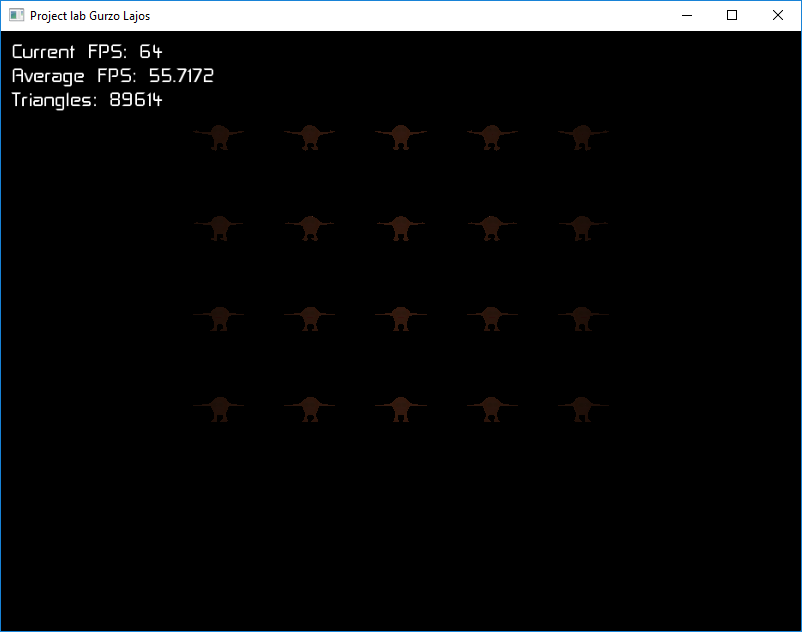
\includegraphics[width=100mm, keepaspectratio]{figures/meas_render_debugdev.png}
\caption{Kiz�r�lag megjelen�t�ssel rendelkez� j�t�kobjektumokn�l fell�p� k�pkockasebess�g hibakeres�
al�l ind�tott, hibakeres�st t�mogat� konfigur�ci� eset�ben.}
\label{fig:MeasRenderDBDev}
\end{figure}

A m�r�st hibakeres� n�lk�l ind�tott, hibakeres�st t�mogat� m�dban is elv�geztem, s j�l l�that�, hogy szignifik�ns k�l�nbs�g nem l�pett fel az
el�bb bemutatott v�ltozathoz k�pest. Az eredm�ny a \figref{MeasRenderDev} �br�n l�that�.

\begin{figure}[!ht]
\centering
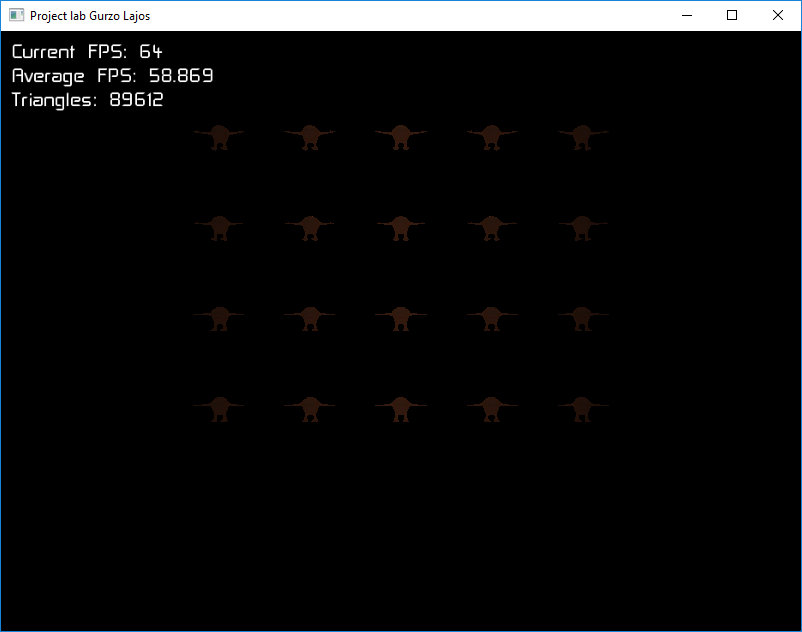
\includegraphics[width=100mm, keepaspectratio]{figures/meas_render_dev.png}
\caption{Kiz�r�lag megjelen�t�ssel rendelkez� j�t�kobjektumokn�l fell�p� k�pkockasebess�g hibakeres�
n�lk�l ind�tott, hibakeres�st t�mogat� konfigur�ci� eset�ben.}
\label{fig:MeasRenderDev}
\end{figure}

Ezt az esetet megvizsg�ltam hibakeres�st nem t�mogat� ford�t�si m�dban is.
Ebben az esetben az �tlagos k�pkockasebess�g nagyj�b�l az �tsz�r�se az el�z� esetek sor�n m�rt �rt�keknek.
A m�r�si eredm�nyt a \figref{MeasRenderRel} �bra szeml�lteti.

\begin{figure}[!ht]
\centering
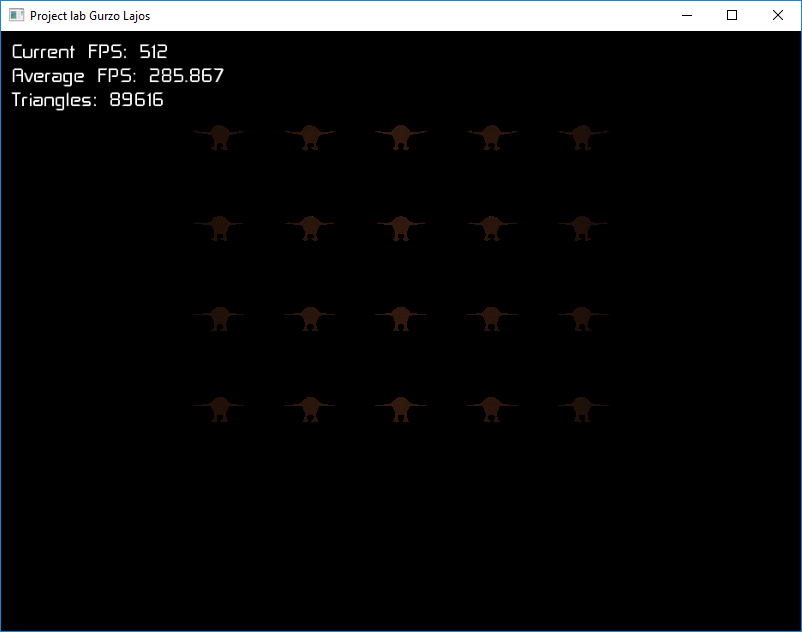
\includegraphics[width=100mm, keepaspectratio]{figures/meas_render_rel.png}
\caption{Kiz�r�lag megjelen�t�ssel rendelkez� j�t�kobjektumokn�l fell�p� k�pkockasebess�g hibakeres�st nem t�mogat� konfigur�ci� eset�ben.}
\label{fig:MeasRenderRel}
\end{figure}

A k�vetkez� m�r�si elrendez�sben ugyanezen j�t�kobjektumokat dinamikus fizikai komponenssel is felruh�ztam.
Az al�bbiakban ezeknek a m�r�seknek az eredm�nyeit k�zl�m.

A program hibakeres� al�l ind�tott hibakeres�st t�mogat� verzi�j�nak m�r�si eredm�nyeit a
\figref{MeasRenderDynamicDBDev} �bra mutatja be.

\begin{figure}[!ht]
\centering
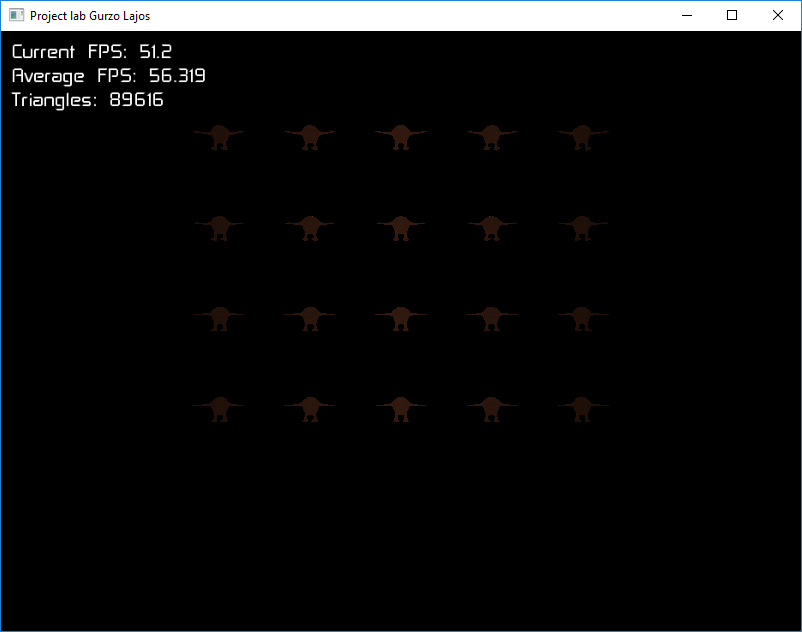
\includegraphics[width=100mm, keepaspectratio]{figures/meas_renderDynamic_debugdev.png}
\caption{Megjelen�t�ssel �s dinamikus fizik�val rendelkez� j�t�kobjektumokn�l fell�p� k�pkockasebess�g
hibakeres� al�l ind�tott hibakeres�st t�mogat� konfigur�ci� eset�ben.}
\label{fig:MeasRenderDynamicDBDev}
\end{figure}

Ugyanezen elrendez�s hibakeres� n�lk�l ind�tott, hibakeres�st t�mogat� konfigur�ci� fut�s�nak eredm�nye
a \figref{MeasRenderDynamicDev} �br�n l�that�.

\begin{figure}[!ht]
\centering
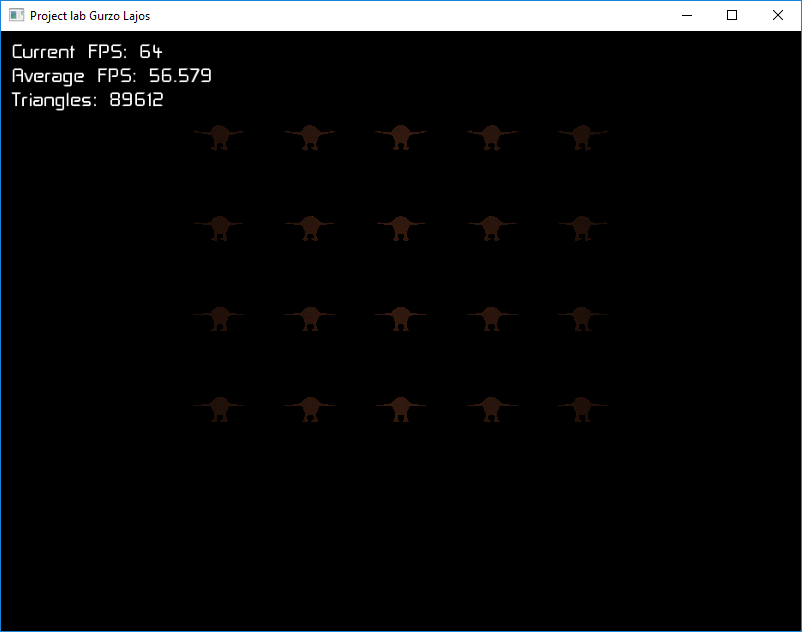
\includegraphics[width=100mm, keepaspectratio]{figures/meas_renderDynamic_dev.png}
\caption{Megjelen�t�ssel �s dinamikus fizik�val rendelkez� j�t�kobjektumokn�l fell�p� k�pkockasebess�g
hibakeres� n�lk�l ind�tott, hibakeres�st t�mogat� program eset�ben.}
\label{fig:MeasRenderDynamicDev}
\end{figure}

Ezt a m�r�st elv�geztem hibakeres�st nem t�mogat� konfigur�ci�n is, melynek eredm�nyeit a \figref{MeasRenderDynamicRel} �bra k�zli.

\begin{figure}[!ht]
\centering
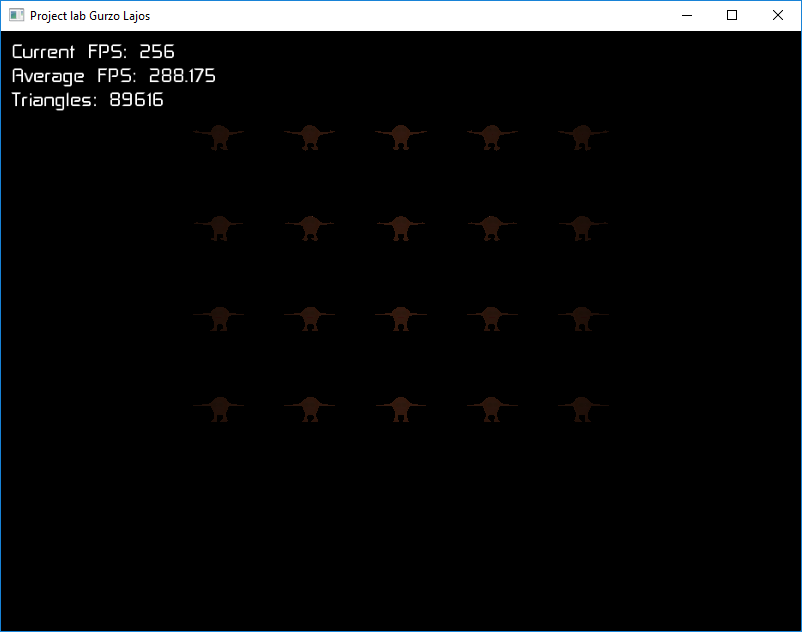
\includegraphics[width=100mm, keepaspectratio]{figures/meas_renderDynamic_rel.png}
\caption{Megjelen�t�ssel �s dinamikus fizik�val rendelkez� j�t�kobjektumokn�l fell�p� k�pkockasebess�g
hibakeres�st nem t�mogat� konfigur�ci� eset�ben.}
\label{fig:MeasRenderDynamicRel}
\end{figure}

A k�vetkez� m�r�seket olyan j�t�kobjektumokon v�geztem, melyek a megjelen�t�s mellett anim�ci�val is rendelkeztek, viszont fizik�val nem.

A program hibakeres� al�l ind�tott, hibakeres�st t�mogat� verzi�j�nak m�r�si eredm�nye a \figref{MeasRenderAnimDBDev} �br�n l�that�.

\begin{figure}[!ht]
\centering
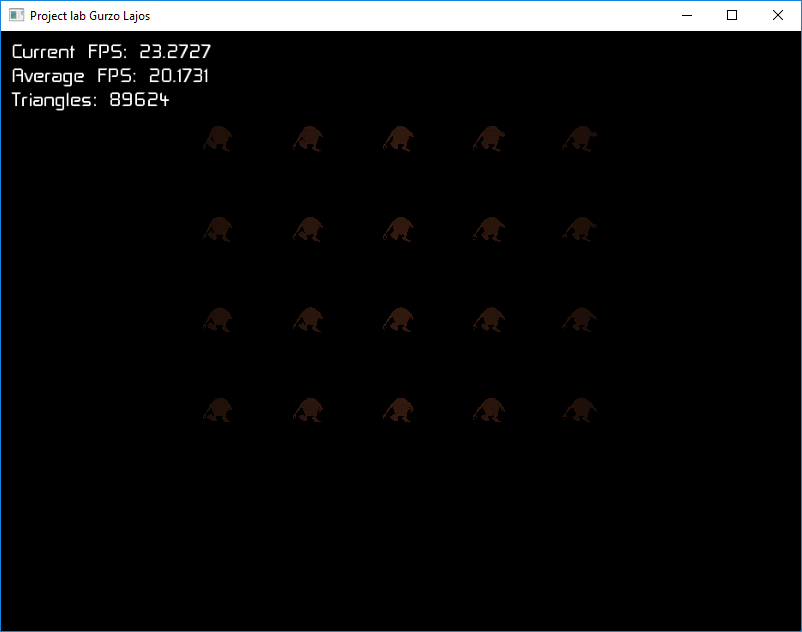
\includegraphics[width=100mm, keepaspectratio]{figures/meas_renderAnim_dbdev.png}
\caption{Megjelen�t�ssel �s anim�ci�val rendelkez� j�t�kobjektumokn�l fell�p� k�pkockasebess�g hibakeres� al�l ind�tott, hibakeres�st t�mogat�
konfigur�ci� eset�ben.}
\label{fig:MeasRenderAnimDBDev}
\end{figure}

Ugyanennek az elrendez�snek a hibakeres� n�lk�l ind�tott, hibakeres�st t�mogat� verzi�j�nak fut�si eredm�nyeit a \figref{MeasRenderAnimDev} �bra szeml�lteti.

\begin{figure}[!ht]
\centering
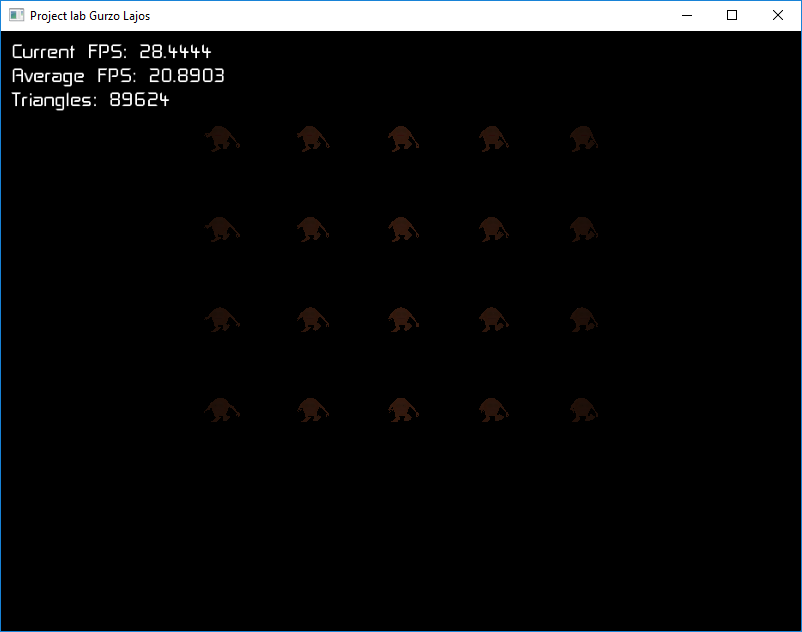
\includegraphics[width=100mm, keepaspectratio]{figures/meas_renderAnim_dev.png}
\caption{Megjelen�t�ssel �s anim�ci�val rendelkez� j�t�kobjektumokn�l fell�p� k�pkockasebess�g hibakeres� n�lk�l ind�tott hibakeres�st t�mogat� program eset�ben.}
\label{fig:MeasRenderAnimDev}
\end{figure}

Ezen elrendez�s hibakeres�st nem t�mogat� programverzi�ja �ltal gener�lt eredm�nyeket a \figref{MeasRenderAnimRel} �bra szeml�lteti.

\begin{figure}[!ht]
\centering
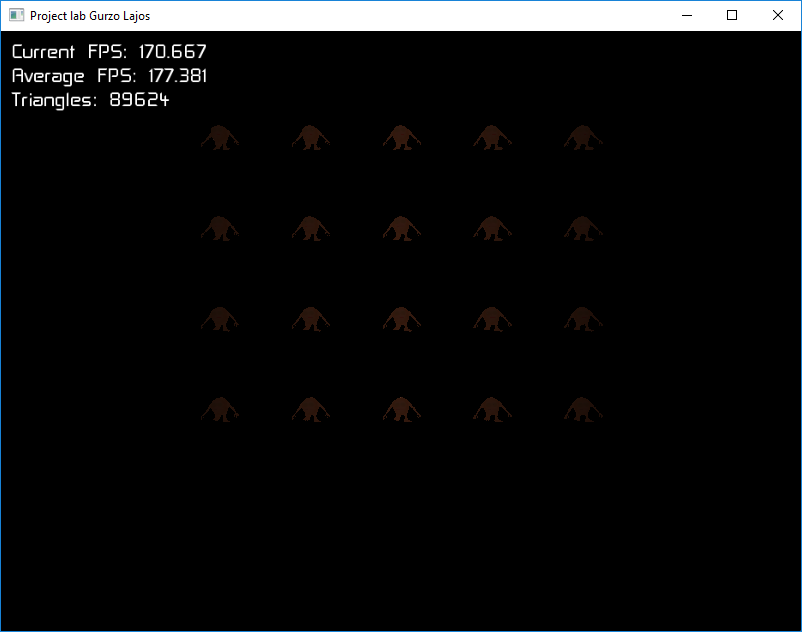
\includegraphics[width=100mm, keepaspectratio]{figures/meas_renderAnim_rel.png}
\caption{Megjelen�t�ssel �s anim�ci�val rendelkez� j�t�kobjektumokn�l fell�p� k�pkockasebess�g hibakeres�st nem t�mogat� program eset�ben.}
\label{fig:MeasRenderAnimRel}
\end{figure}

V�g�l olyan j�t�kobjektumokon v�geztem a m�r�seket, melyek a megjelen�t�s mellett pontf�nyforr�ssal rendelkeznek, �s semmi m�ssal.
Megjegyzend�, hogy ennek hat�s�ra t�zszeres�re n�tt a megjelen�tend� h�romsz�gek sz�ma, ahogy azt a k�perny�k�pekb�l is l�tni lehet.

A hibakeres� al�l ind�tott, hibakeres�st t�mogat� konfigur�ci� fut�si eredm�nyeit az \figref{MeasRenderLightDBDev} �bra szeml�lteti.

\begin{figure}[!ht]
\centering
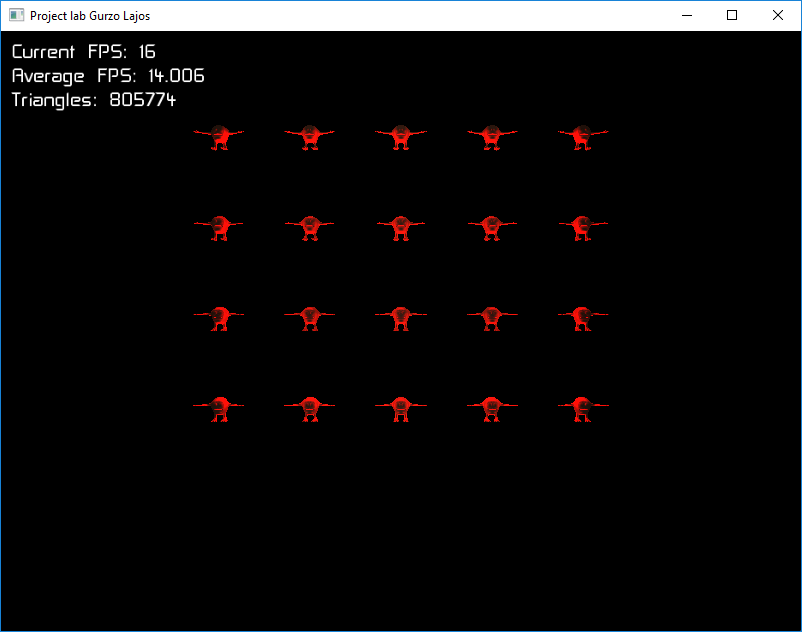
\includegraphics[width=100mm, keepaspectratio]{figures/meas_renderLight_dbdev.png}
\caption{Megjelen�t�ssel �s pontf�nyforr�ssal rendelkez� j�t�kobjektumokn�l fell�p� k�pkockasebess�g hibakeres� al�l ind�tott, hibakeres�st t�mogat� program eset�ben.}
\label{fig:MeasRenderLightDBDev}
\end{figure}

A hibakeres� n�lk�l ind�tott hibakeres�st t�mogat� fut�s eredm�nyeit az \figref{MeasRenderLightDev} �bra mutatja.

\begin{figure}[!ht]
\centering
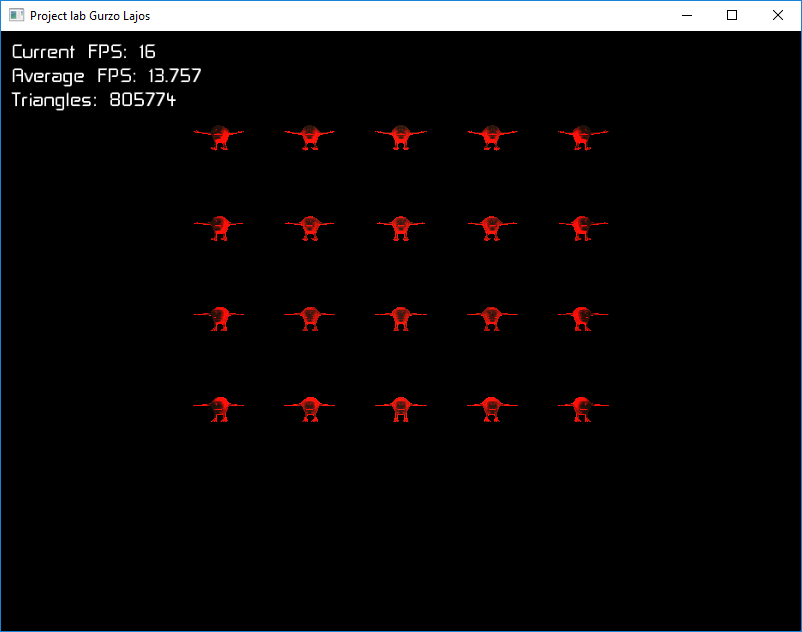
\includegraphics[width=100mm, keepaspectratio]{figures/meas_renderLight_dev.png}
\caption{Megjelen�t�ssel �s pontf�nyforr�ssal rendelkez� j�t�kobjektumokn�l fell�p� k�pkockasebess�g hibakeres� n�lk�l ind�tott hibakeres�st t�mogat� program eset�ben.}
\label{fig:MeasRenderLightDev}
\end{figure}

A hibakeres�st nem t�mogat� verzi�nak az eredm�nyeit az \figref{MeasRenderLightRel} �bra foglalja mag�ban.

\begin{figure}[!ht]
\centering
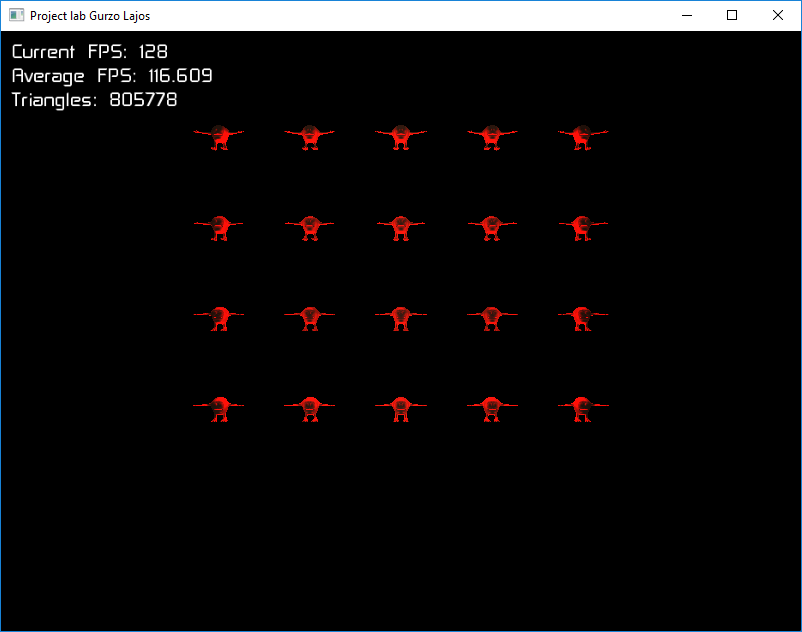
\includegraphics[width=100mm, keepaspectratio]{figures/meas_renderLight_rel.png}
\caption{Megjelen�t�ssel �s pontf�nyforr�ssal rendelkez� j�t�kobjektumokn�l fell�p� k�pkockasebess�g hibakeres�st nem t�mogat� konfigur�ci� eset�ben.}
\label{fig:MeasRenderLightRel}
\end{figure}

A m�r�si konfigur�ci�k �s azok eredm�nyeinek ismertet�se ut�n az eredm�nyek �sszefoglal�s�t �s �rtelmez�s�t teszem meg.

Az \tabref{MeasDBDevTable}-es t�bl�zat foglalja �ssze a hibakeres� al�l futtatott, hibakeres�st t�mogat� konfigur�ci� fut�si eredm�nyeit.

\begin{table}[ht]
	\footnotesize
	\centering
	\caption{A hibakeres� al�l futtatott hibakeres�st t�mogat� programok fut�sainak eredm�nyei.} \label{tab:MeasDevTableDesc}
	\begin{tabular}{ | l | c | c | c | c | }
	\hline
				& Megjelen�t�s & Fizika & Anim�ci� & F�nyforr�s \\ \hline
	�tlagos FPS & 55.72 & 56.32 & 20.17 & 14 \\ \hline
	H�romsz�gek & 89614 & 89616 & 89624 & 805774 \\ \hline
	\end{tabular}
	\label{tab:MeasDBDevTable}
\end{table}

A \tabref{MeasDevTable}-as t�bl�zat a hibakeres� n�lk�l futtatott, hibakeres�st t�mogat� konfigur�ci� fut�si eredm�nyeit foglalja �ssze.

\begin{table}[ht]
	\footnotesize
	\centering
	\caption{A hibakeres� n�lk�l futtatott hibakeres�st t�mogat� konfigur�ci� fut�sainak eredm�nyei.} \label{tab:MeasDevTableDesc}
	\begin{tabular}{ | l | c | c | c | c | }
	\hline
				& Megjelen�t�s & Fizika & Anim�ci� & F�nyforr�s \\ \hline
	�tlagos FPS & 58.87 & 56.58 & 20.89 & 13.76 \\ \hline
	H�romsz�gek & 89612 & 89612 & 89624 & 805774 \\ \hline
	\end{tabular}
	\label{tab:MeasDevTable}
\end{table}

A \tabref{MeasRelTable}-es t�bl�zat a hibakeres�st nem t�mogat� konfigur�ci� fut�si eredm�nyeit tartalmazza.

\begin{table}[ht]
	\footnotesize
	\centering
	\caption{A hibakeres�st nem t�mogat� konfigur�ci� fut�sainak eredm�nyei.} \label{tab:MeasDevTableDesc}
	\begin{tabular}{ | l | c | c | c | c | }
	\hline
				& Megjelen�t�s & Fizika & Anim�ci� & F�nyforr�s \\ \hline
	�tlagos FPS & 285.87 & 288.18 & 177.38 & 116.61 \\ \hline
	H�romsz�gek & 89616 & 89616 & 89624 & 805778 \\ \hline
	\end{tabular}
	\label{tab:MeasRelTable}
\end{table}

A m�r�si eredm�nyekb�l j�l l�that�, hogy a rendszeremben a sz�k keresztmetszetet a megjelen�t�shez kapcsol�d�
funkcionalit�sok jelentik. Ezt m�g jobban al�t�masztand� k�sz�tettem egy teljes�tm�nym�r�st a Visual Studio 2015
be�p�tett teljes�tm�ny profiloz� eszk�z�vel. A m�r�st a demonstr�ci�s alkalmaz�son v�geztem el.
Ennek az eredm�nye a \figref{ProfilingDBDev} �br�n l�that�:

\begin{figure}[!ht]
\centering
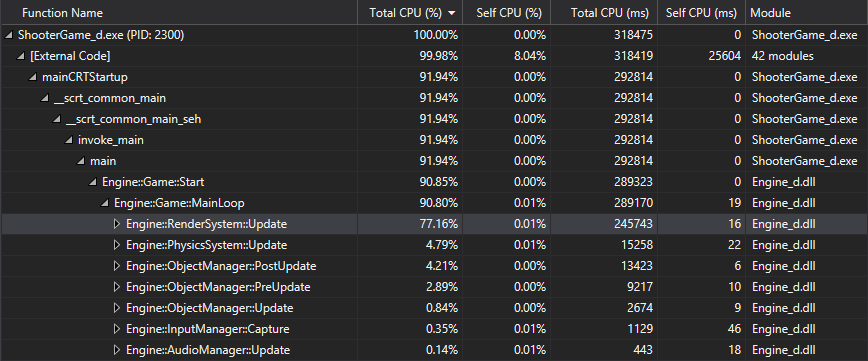
\includegraphics[width=90mm, keepaspectratio]{figures/profiling_debugdev.png}
\caption{A rendszerben lev� sz�k keresztmetszet a megjelen�t�s.}
\label{fig:ProfilingDBDev}
\end{figure}

%----------------------------------------------------------------------------
\chapter{�sszefoglal�s �s kitekint�s}
%----------------------------------------------------------------------------
igaz�b�l a legl�nyegesebb dolog a demonstr�ci�s alkalmaz�s, ha azt t�l neh�z volt meg�rni, akkor
nem lett el�g j� a motor

tovabbfejlesztesi lehetosegek:
halozat, tobbszalusitas, szkripteles, grafikus palyaszerkeszto (xml generalasa az iras helyett), ...

%\listoffigures\addcontentsline{toc}{chapter}{�br�k jegyz�ke}
%\listoftables\addcontentsline{toc}{chapter}{T�bl�zatok jegyz�ke}

\bibliography{mybib}
\addcontentsline{toc}{chapter}{Irodalomjegyz�k}
\bibliographystyle{plain}

%----------------------------------------------------------------------------
\appendix
%----------------------------------------------------------------------------
\chapter*{F�ggel�k}\addcontentsline{toc}{chapter}{F�ggel�k}
\setcounter{chapter}{6}  % a fofejezet-szamlalo az angol ABC 6. betuje (F) lesz
\setcounter{equation}{0} % a fofejezet-szamlalo az angol ABC 6. betuje (F) lesz
\numberwithin{equation}{section}
\numberwithin{figure}{section}
\numberwithin{lstlisting}{section}
%\numberwithin{tabular}{section}

CMake szkriptek tartalma

XML leiro fajl tartalma (prefab peldanyositas, fontosabb komponensek leirasa stb.)


\label{page:last}
\end{document}
